\section{Extended Comparison with Prior Work}
\subsection{KV Cache Optimization}
\label{appendx: kv opt}
\paragraph{Multi-tiered KV cache management.}
To alleviate GPU memory pressure, systems such as Pensieve~\citep{Yu_2025}, Continuum~\cite{li2025continuumefficientrobustmultiturn}, Strata~\citep{xie2025stratahierarchicalcontextcaching}, and ShadowKV~\citep{sun2025shadowkvkvcacheshadows} exploit the hardware memory hierarchy, comprising GPU HBM, CPU DRAM, and NVMe SSD for KV cache management. These tiered caching mechanisms mitigate transient preemption by offloading inactive KV states to lower-tier storage and prefetching them back to GPU upon request resumption. However, the practical efficiency of these methods is fundamentally constrained by the inter-tier bandwidth between device and host memory. In high-frequency agentic workflows, the overhead of frequent swap-in and swap-out cycles often negates the benefits of multi-tier caching as shown in \autoref{sec:experiments}.

% \textbf{Predictive and Workflow-Aware Context Persistence.}
% To mitigate the overhead of KV-cache re-prefill, recent works’ KV cache management has shifted from reactive eviction to proactive persistence. Systems like Continuum~\citep{li2025continuumefficientrobustmultiturn} utilize temporal heuristics to predict request arrival intervals and pin active caches accordingly.

% However, these frameworks primarily target dynamic serving scenarios, prioritizing step-wise and end-to-end latency. Furthermore, their reliance on semantic tool classification fails to account for the significant intra-class variance present in remote model API calling and compilers.

\paragraph{Distributed KV cache management.}
Distributed management of agentic states introduces significant complexity to KV cache eviction and preemption policies. While systems like BanaServe~\citep{he2025banaserveunifiedkvcache} and LMCache~\citep{liu2025lmcacheefficientkvcache} enable KV cache transfer across DP nodes, their performance in large-batch agentic serving and rollout is often constrained by limited interconnect bandwidth. The strong intra-program dependencies in agentic workflows necessitate frequent state transferring without program-level management, which can easily saturate the network during serving or rollout.

To bypass these bandwidth bottlenecks, standard inference systems like vLLM KV-aware router~\citep{vllm_kvaware_routing} and SGLang Model Gateway~\citep{zheng2024sglangefficientexecutionstructured} employ KV-aware routing policies that pin requests to specific nodes based on prefix locality or session ID. Similarly, Vortex~\citep{yuan2025vortexovercomingmemorycapacity} introduces session-aware prefetching to minimize cross-node data transfer latency. However, these approaches lack the capability to dynamically migrate active program states between DP nodes. This absence of workload transfer leads to severe memory utilization imbalance across the cluster, shown in \autoref{fig:dp unbalance}. Nodes hosting long-running agentic programs cannot offload states to idle peers, resulting in fragmented resource utilization and degraded aggregate throughput.

\subsection{Extended experiment results on KV cache optimization}
\label{sec: pd+offload}
\paragraph{Experiments on KV cache offloading.}
We investigated KV cache offloading by using LMcache~\cite{liu2025lmcacheefficientkvcache} as a potential remedy for capacity constraints. While offloading theoritically extends effective memory space by utilizing CPU or SSD storage, our implementation with vLLM + LMcache reveals a critical bottleneck: the PCIe bandwidth is insufficient to sustain the high-frequency context switching and large-volume data transfers inherent to agentic workloads. As demonstrated in \autoref{fig:lmcache}, when serving the GLM-4.6 model~\cite{5team2025glm45agenticreasoningcoding} with the mini-SWEAgent framework~\cite{yang2024sweagentagentcomputerinterfacesenable}, the latency penalty from frequent swap-in and swap-out operations negates the memory capacity benefits, resulting in severe throughput degradation under heavy agentic workloads.

\paragraph{Experiments on Prefill-Decode (PD) disaggregation.}
We also explored PD disaggregation~\cite{zhong2024distservedisaggregatingprefilldecoding}, a standard optimization for chatbot serving by isolating the decoding phase from prefill interference. However, when applied to agentic workloads characterized by continuous context growth, we observe that PD disaggregation \textbf{\textit{exacerbates}} thrashing. By partitioning the cluster into prefill-only and decode-only nodes, the effective HBM pool available for handling prefill is significantly smaller than that in a unified architecture. This memory fragmentation causes the system to hit capacity limits and trigger thrashing at much lower concurrency levels, as shown in \autoref{fig:throughput_pd}. These results demonstrate that generic architectural optimizations cannot substitute for a program-centric scheduler that actively manages the working set.

\begin{figure}[b]
    \centering
    % --- 左边的图 ---
    % 将容器宽度设为 0.49 (占左半边空间)
    \begin{subfigure}[b]{0.49\linewidth}
        \centering
        % 图片宽度设为 0.6 (相对于容器)，实际效果约为页面的 0.3
        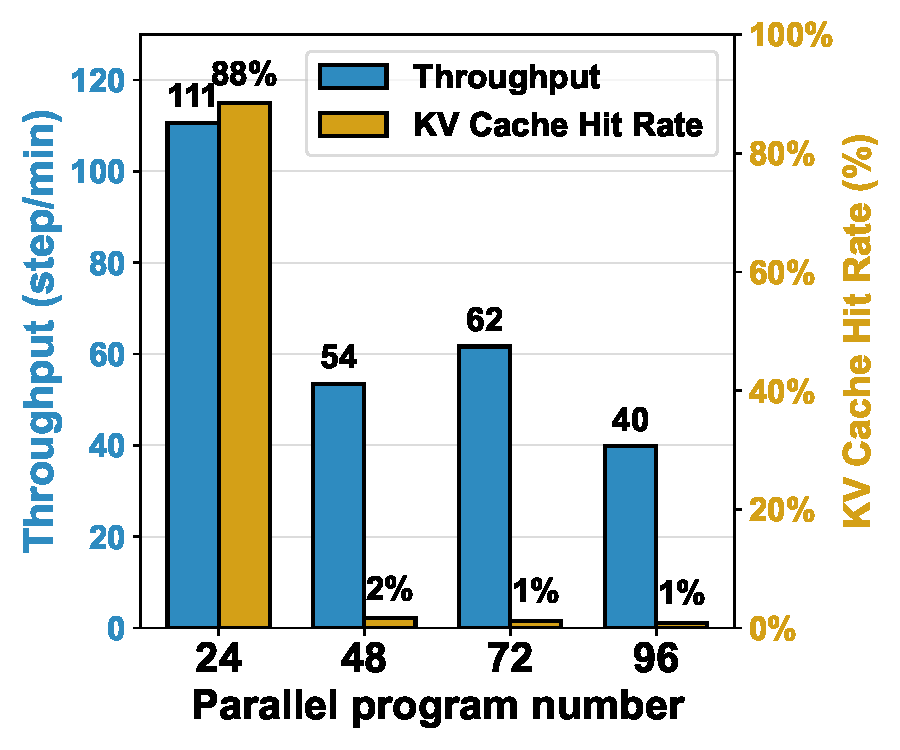
\includegraphics[width=0.99\linewidth]{Figures/lmcache.pdf}
        \caption{KV Cache Hit Rate with LMCache Offloading}
        \label{fig:lmcache}
    \end{subfigure}
    \hfill % 在两个 0.49 的盒子中间填充微小空隙
    % --- 右边的图 ---
    \begin{subfigure}[b]{0.49\linewidth}
        \centering
        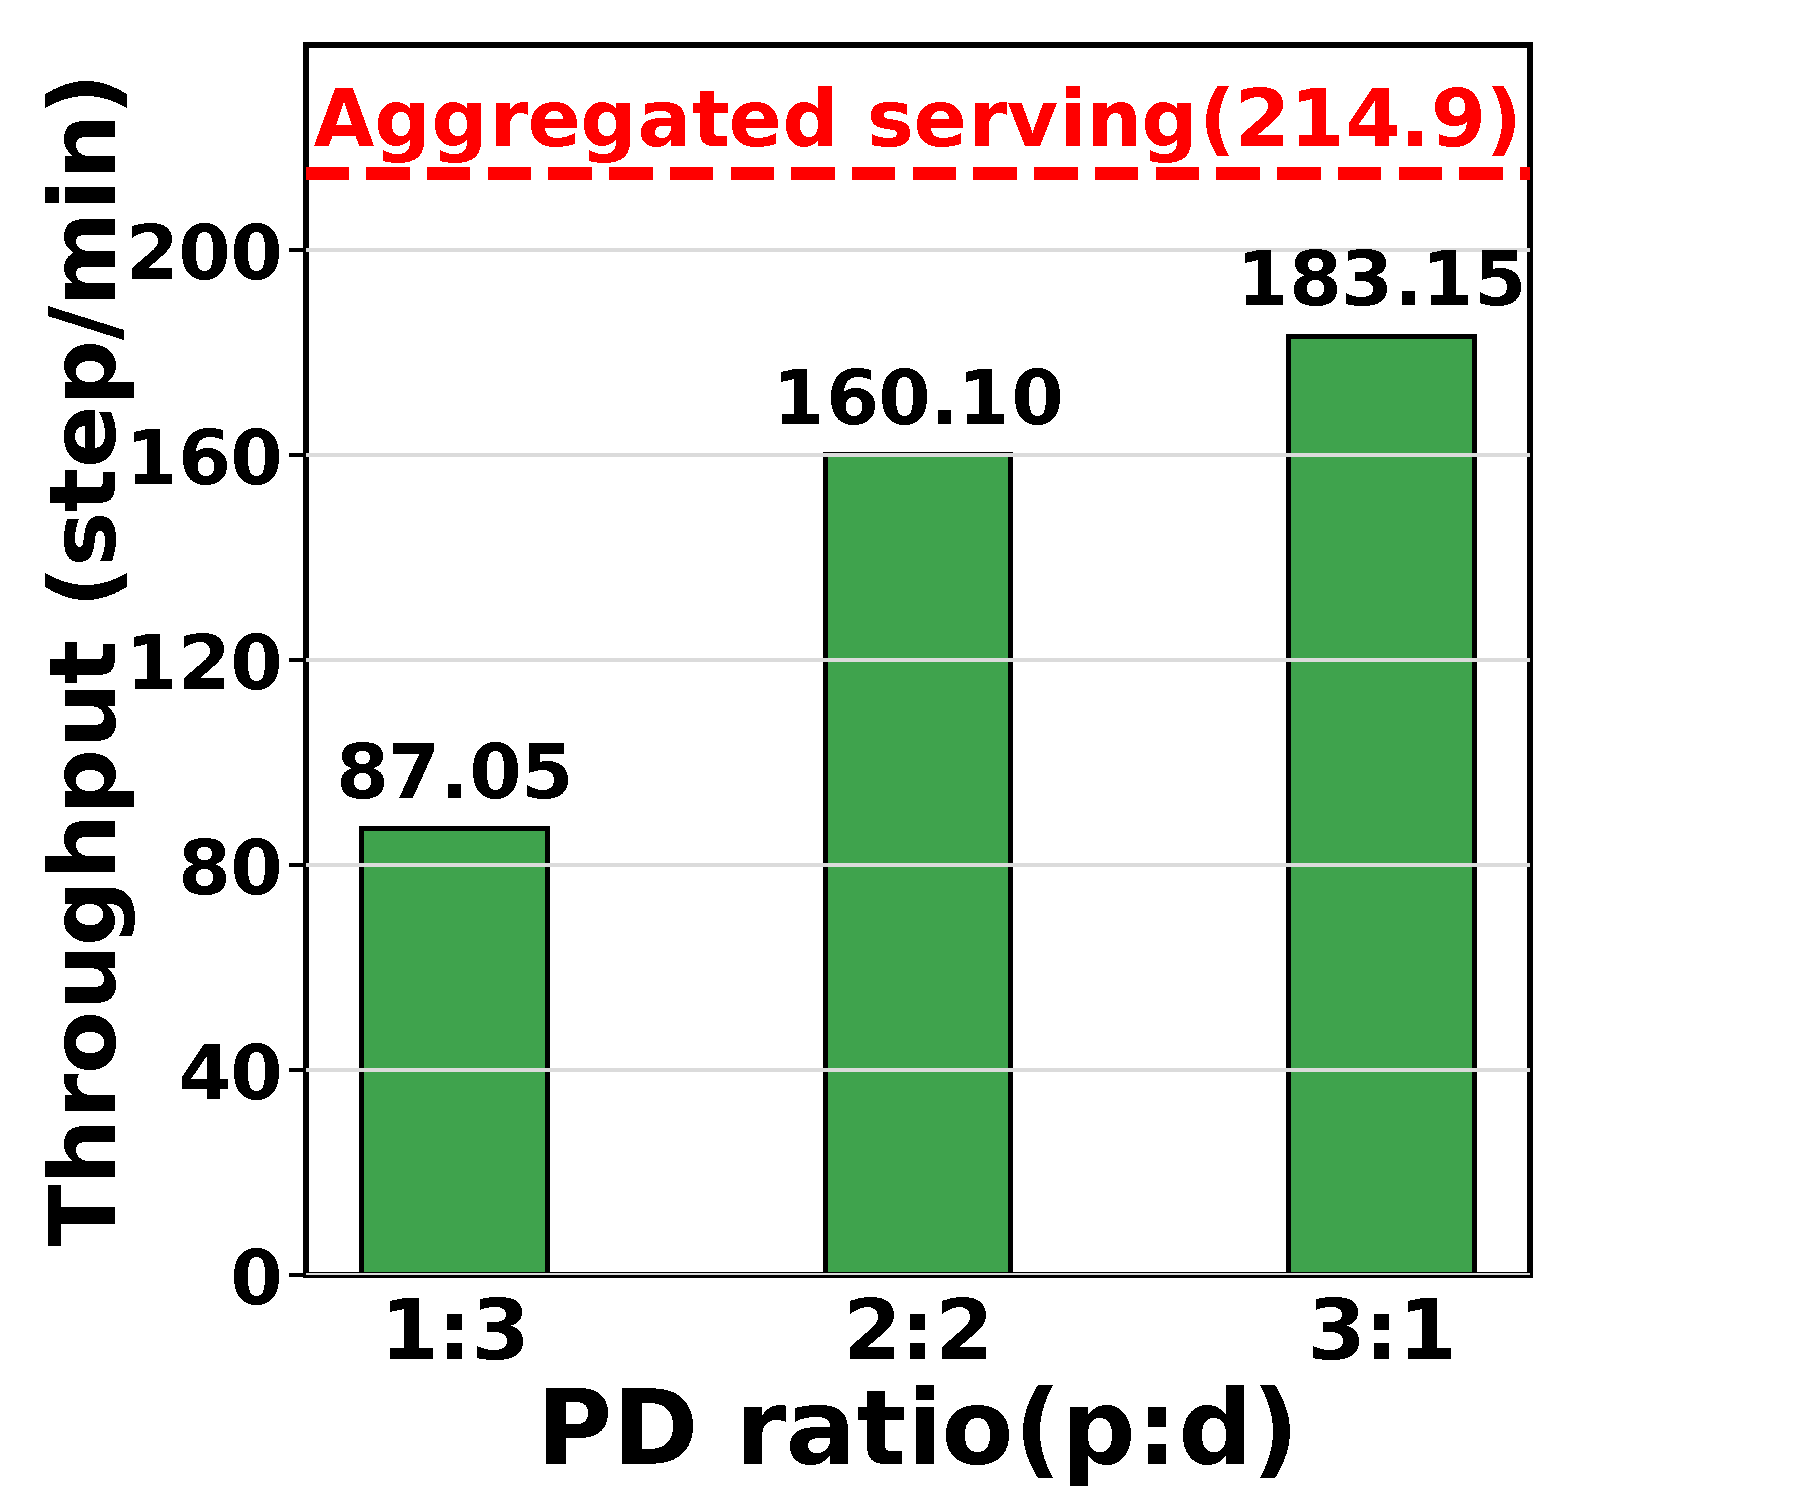
\includegraphics[width=0.99\linewidth]{Figures/throughput_vs_pd_ratio.pdf}
        \caption{Throughput v.s. Prefill-Only/Decode-Only Node Ratio}
        \label{fig:throughput_pd}
    \end{subfigure}

    \caption{Ablation study on KV cache offloading and Prefill-Decode (PD) disaggregation}
    \label{fig:both_figures}
\end{figure}



\subsection{Scaling up agentic workflows}
\label{sec:rl_scale}
\textbf{Heterogeneous resource allocation and scheduling.}
To orchestrate multi-turn agent-environment interactions at scale, recent systems such as MegaFlow~\cite{zhang2026megaflow}, RollArt~\cite{gao2025rollart,wang2025let}, AgentRL~\cite{zhang2025agentrl}, and VerlTool~\cite{jiang2025verltool} decouple model inference from environment execution. While these frameworks effectively scale environment concurrency via specialized services, they exhibit the inherent limitations of coarse-grained disaggregation. By treating the inference engine and tool executor as isolated black boxes, these systems lack unified resource management and are unable to coordinate KV cache lifecycles with the environment execution. Without fine-grained scheduling at program-level, disaggregation-based approaches waste KV cache reuse potential in agentic workloads, yielding sub-optimal throughput.

\newpage

\section{System Portability and Interface Abstraction.}
\label{app:easy_intergrate}
\subsection{Middleware Architecture and Unified Interfaces.}
\noindent \ouralg serves as \textbf{a program-aware runtime layer} that mediates between agent control flow and backend inference engines via a program-level abstraction. The scheduler controls program state transitions based on the abstracted \texttt{ProgramState} (see Table~\ref{tab:program-state}) together with the backend cache capacity view (see Table~\ref{tab:backend-state}). Meanwhile, each program binds only to the endpoint and does not depend on the concrete backend implementation.

\subsection{Why program ID matters.}

While the standard \textbf{session ID} serves as a routing label, \textbf{the program ID is used by our system to check the workflow metadata.} This visibility is critical: it allows the scheduler to distinguish valid tool-wait times from idle sessions, enabling smart preemption strategies that session-based baselines cannot support.

\subsection{Low-overhead adoption of the ThunderAgent.}
Figure~\ref{fig:router-minimal-changes} shows that adopting ThunderAgent \textbf{only requires} attaching \texttt{program\_id} to requests (for both LLM inference and tool execution) and sending an explicit release signal with \texttt{program\_id} when a program ends.
The \texttt{program\_id} tags each request with its own program instance for scheduling, while the
release signal allows ThunderAgent to reclaim per-program resources after termination.
\textbf{All other request fields and the OpenAI-style API surface remain unchanged.}

%pipeline contradiction


%program state table
\begin{table}[!htbp]
\centering
\footnotesize
\setlength{\tabcolsep}{3pt}
\renewcommand{\arraystretch}{1.05}

\begin{subtable}[t]{0.56\linewidth}
\centering
\begin{tabular}{@{} l l p{0.54\linewidth} @{}}
\toprule
\textbf{Field} & \textbf{Type} & \textbf{Meaning} \\
\midrule
\multicolumn{3}{@{}l}{\textbf{ProgramState}} \\
\addlinespace[2pt]
\texttt{status}        & ProgramStatus & Current lifecycle state. \\
\texttt{backend\_url}  & str           & Assigned backend endpoint. \\
\texttt{step\_count}   & int           & Executed steps so far. \\
\texttt{total\_tokens} & int           & Total tokens over full history. \\
\bottomrule
\end{tabular}
\subcaption{ProgramState fields.}
\label{tab:program-state}
\end{subtable}
\hfill
\begin{subtable}[t]{0.42\linewidth}
\centering
% key change: fixed-width first column + explicit gap + remaining-width second column
\begin{tabular}{@{} >{\raggedright\arraybackslash}p{0.34\linewidth}
                @{\hspace{10pt}}
                >{\raggedright\arraybackslash}p{0.56\linewidth} @{}}
\toprule
\textbf{Status} & \textbf{Meaning} \\
\midrule
\multicolumn{2}{@{}l}{\textbf{ProgramStatus}} \\
\addlinespace[2pt]
\texttt{REASONING} & On-GPU inference. \\
\texttt{ACTING}    & Off-GPU tool exec. \\
\texttt{PAUSED}    & In global paused waiting set. \\
\texttt{STOPPED}   & Released; resources reclaimed. \\
\bottomrule
\end{tabular}
\subcaption{ProgramStatus semantics.}
\label{tab:program-status}
\end{subtable}

\caption{Program state and status definitions.}
\label{tab:program-state-status}
\end{table}

%backend state table
\begin{table}[!htbp]
\centering
\footnotesize
\setlength{\tabcolsep}{3pt}
\renewcommand{\arraystretch}{1.05}

\begin{tabular}{@{} l l p{6.2cm} @{}}
\toprule
\textbf{Field} & \textbf{Type} & \textbf{Meaning} \\
\midrule
\multicolumn{3}{@{}l}{\textbf{BackendState}} \\
\addlinespace[2pt]
\texttt{url} & str & Backend endpoint. \\
\texttt{healthy} & bool & Health flag for scheduling. \\
\texttt{cache\_config} & Optional[CacheConfig] & Static cache configuration (fetched at startup). \\
\texttt{active\_program\_tokens} & int & Active token footprint on this backend. \\
\bottomrule
\end{tabular}

\vspace{6pt} % <-- increase to push caption further down
\caption{Key fields of BackendState.}
\label{tab:backend-state}

\end{table}

\begin{figure}[!htbp]
\centering

\begin{minipage}[t]{0.485\linewidth}
\centering
\textbf{Only inference backend (e.g., vLLM/SGLang)}\\[-2pt]
\begin{tcolorbox}[
  colback=black!3,
  colframe=black!35,
  boxrule=0.4pt,
  arc=1.2pt,
  left=4pt,right=4pt,top=3pt,bottom=3pt
]
\begin{lstlisting}[style=req]
(*@\textcolor{blue!70!black}{\# 1) LLM request}@*)
chat_completion(model_id, messages, extrabody)

(*@\textcolor{blue!70!black}{\# 2) Tool execution}@*)
run_tool(command, sandbox)

(*@\textcolor{blue!70!black}{\# 3) Program end}@*)
# (no explicit release)
\end{lstlisting}
\end{tcolorbox}
\end{minipage}
\hfill
\begin{minipage}[t]{0.485\linewidth}
\centering
\textbf{With ThunderAgent}\\[-2pt]
\begin{tcolorbox}[
  colback=black!3,
  colframe=black!35,
  boxrule=0.4pt,
  arc=1.2pt,
  left=4pt,right=4pt,top=3pt,bottom=3pt
]
\begin{lstlisting}[style=req]
(*@\textcolor{orange!80!black}{\# 1) LLM request}@*)
extrabody[(*@\textbf{"program\_id"}@*)] = "PID"
chat_completion(model_id, messages, extrabody)

(*@\textcolor{orange!80!black}{\# 2) Tool execution}@*)
run_tool(command, sandbox, (*@\textbf{program\_id="PID"}@*))

(*@\textcolor{orange!80!black}{\# 3) Program end (explicit release)}@*)
POST /programs/release
{ (*@\textbf{"program\_id"}@*): "PID" }
\end{lstlisting}
\end{tcolorbox}
\end{minipage}

\caption{\textbf{Only three changes are required to use the ThunderAgent.}}
\label{fig:router-minimal-changes}
\end{figure}






\newpage
\section{Tool execution time variability.}
\label{app:tool_var}

\noindent\textbf{Practical agent tool calls are hard to characterize and often unpredictable.} In some code-centric settings (e.g., serving SWE-Bench~\citep{jimenez2024swebenchlanguagemodelsresolve} with SWE-agent~\citep{yang2024sweagentagentcomputerinterfacesenable} or OpenHands~\citep{wang2025openhandsopenplatformai}), agents primarily invoke local, lightweight tools, and tool latency is relatively stable with low variance. However, in broader and more realistic scenarios, e.g., serving HLE~\citep{phan2025humanitysexam} with ToolOrchestra~\citep{su2025toolorchestraelevatingintelligenceefficient}, the workload relies more heavily on remote-service tools (Table~\ref{tab:tool-buckets}), making tool execution time volatile and difficult to predict. This volatility largely stems from factors external to the agent runtime, such as network jitter, backend load and queuing delays, and rate limiting, which can vary across requests and over time.

We empirically confirm this behavior in Figure~\ref{fig:tool_time}. For remote-service tools (and some execution tools), the gap between the median and tail quantiles is large: p95 and p99 are substantially higher than the median, and the tail can extend to tens or even hundreds of seconds. This suggests that tool latency in these settings lacks a stable central tendency; instead, heavy-tailed behavior dominates, \textbf{making tool latency prediction intrinsically brittle in practice.}

Given the unpredictability of tool execution, underestimation wastes pinned cache capacity while still triggering premature KV eviction, causing thrashing upon resume. Overestimation, in contrast, may lead to unnecessary eviction of programs' KV that should have remained pinned. Even if tool runtimes were perfectly predictable, existing methods such as continuum~\cite{li2025continuumefficientrobustmultiturn} still decide whether to keep the KV cache pinned using a static, threshold-based rule. In contrast, ThunderAgent builds \textbf{a complete cost-modeling framework} and \textbf{dynamically trades off} $\text{Cost}_{\text{recompute}}$ and $\text{Cost}_{\text{caching}}$.








\begin{table}[!htbp]
\centering
\small
\setlength{\tabcolsep}{8pt}
\begin{tabular}{l l l}
\toprule
\textbf{Tool bucket} & \textbf{Role} & \textbf{Primary variability source} \\
\midrule
\texttt{HLE-search} & Retrieve evidence & Remote service(Network latency/Rate limits) \\
\texttt{HLE-enhance-reasoning} & Model-as-a-tool call & Remote service \\
\texttt{HLE-answer} & Final generation & Local LLM inference \\
\midrule
\texttt{SAB-execute\_bash} & Shell execution & Sandbox and I/O \\
\texttt{SAB-execute\_ipython\_cell} & Python cell execution & Program runtime \\
\texttt{SAB-str\_replace\_editor} & File edit & Local filesystem \\
\texttt{SAB-task\_tracker} & Task state tracking & Local filesystem \\
\bottomrule
\end{tabular}
\vspace{6pt}
\caption{Tool buckets.}
\label{tab:tool-buckets}
\end{table}





\begin{figure*}[]
  \centering

  % ===================== Row 1: HLE (3/3 filled) =====================
  \begin{subfigure}[t]{0.32\textwidth}
    \centering
    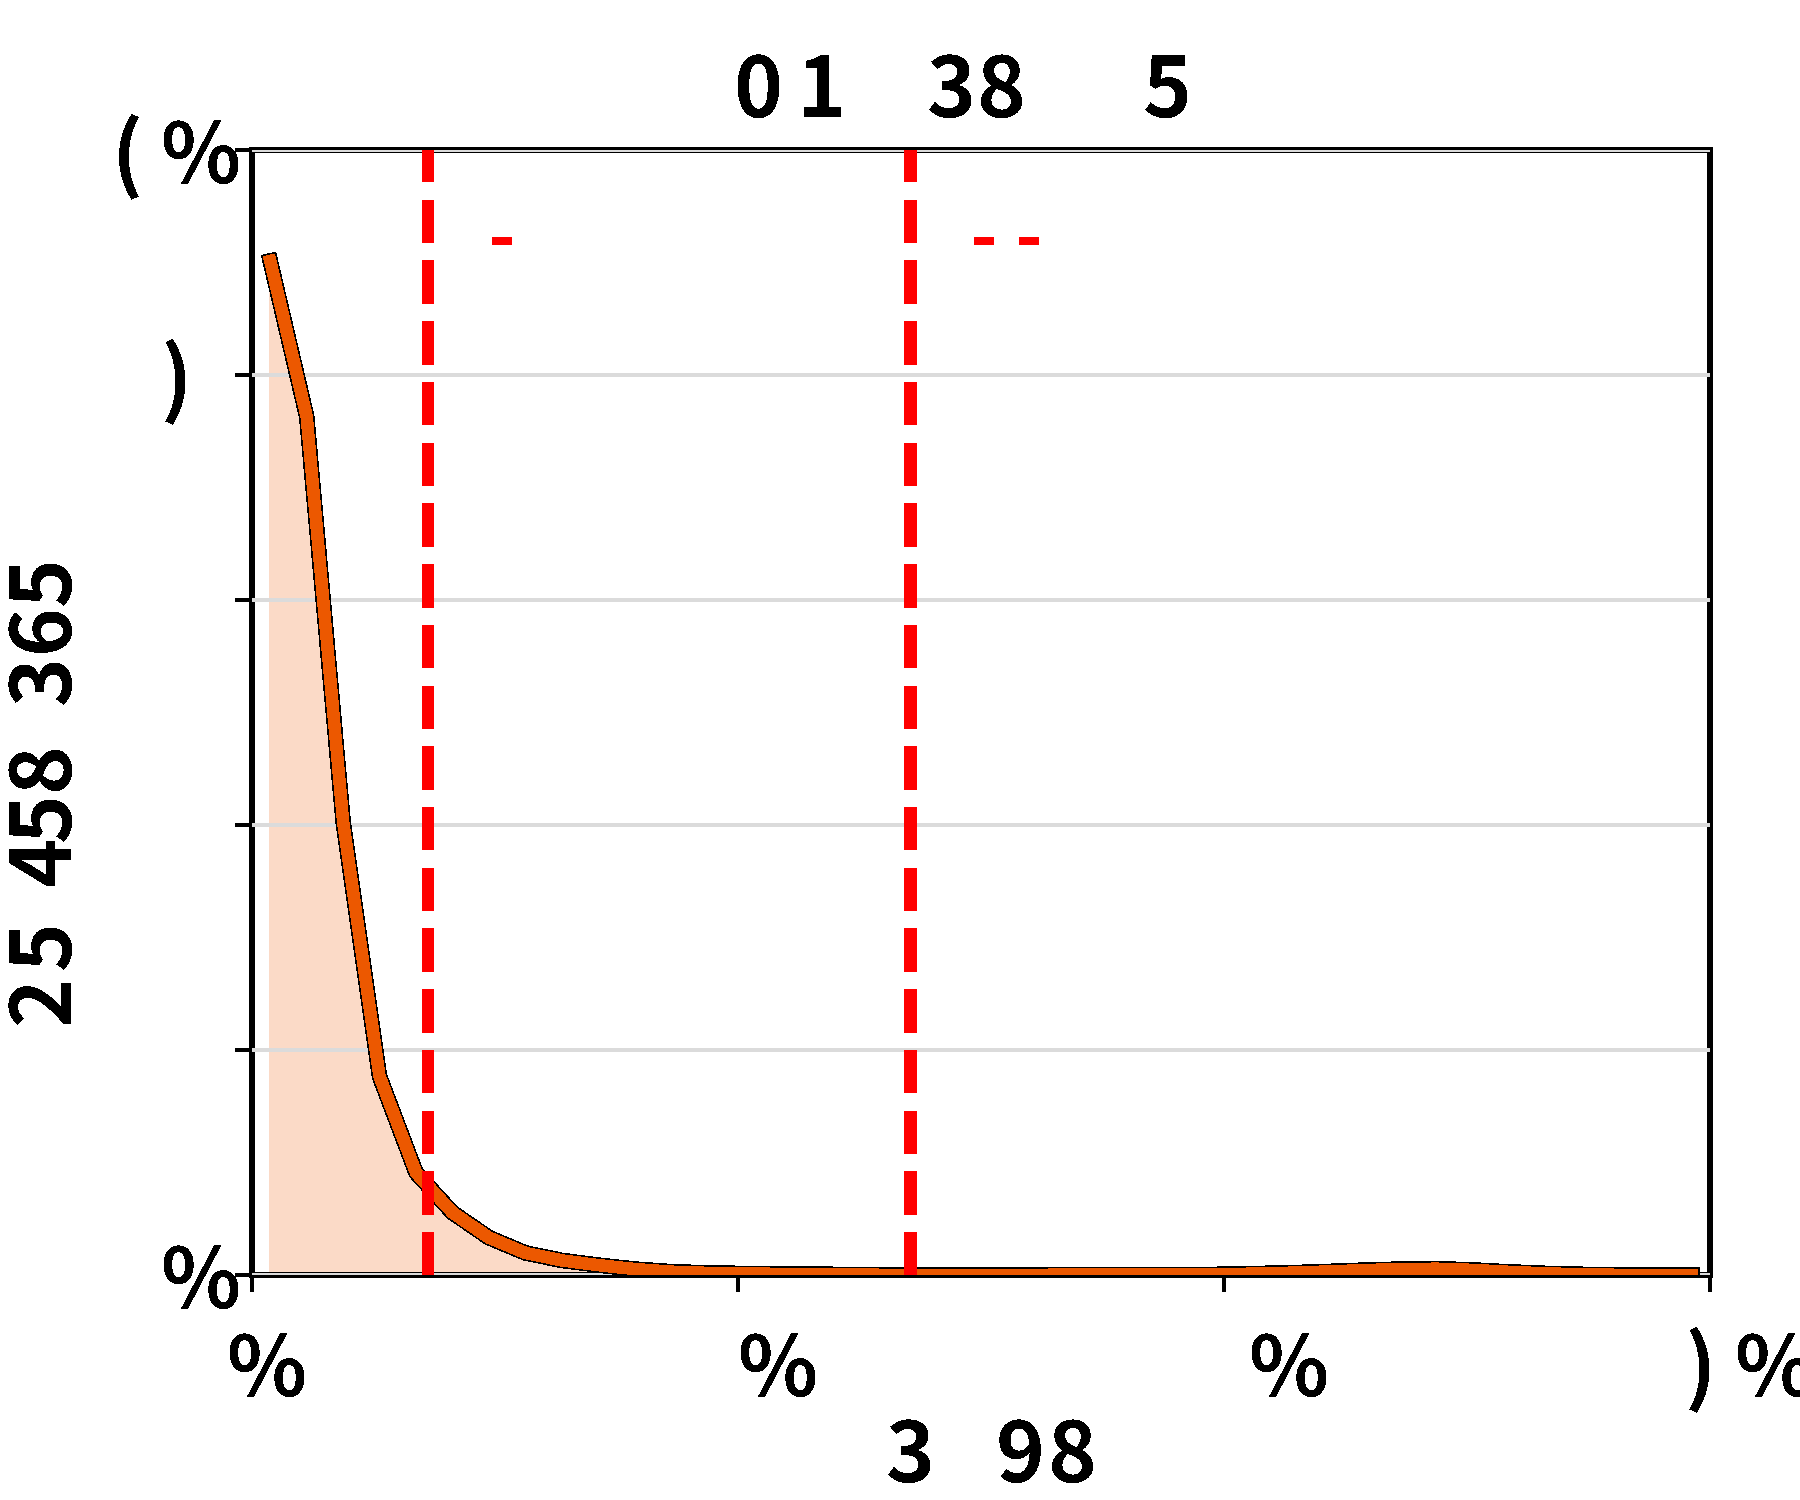
\includegraphics[width=0.8\linewidth ]{Figures/appendix_figs/hle_answer_latency_dist.pdf} % (a) optional
    \label{fig:hle_answer_latency}
  \end{subfigure}\hfill
  \begin{subfigure}[t]{0.32\textwidth}
    \centering
    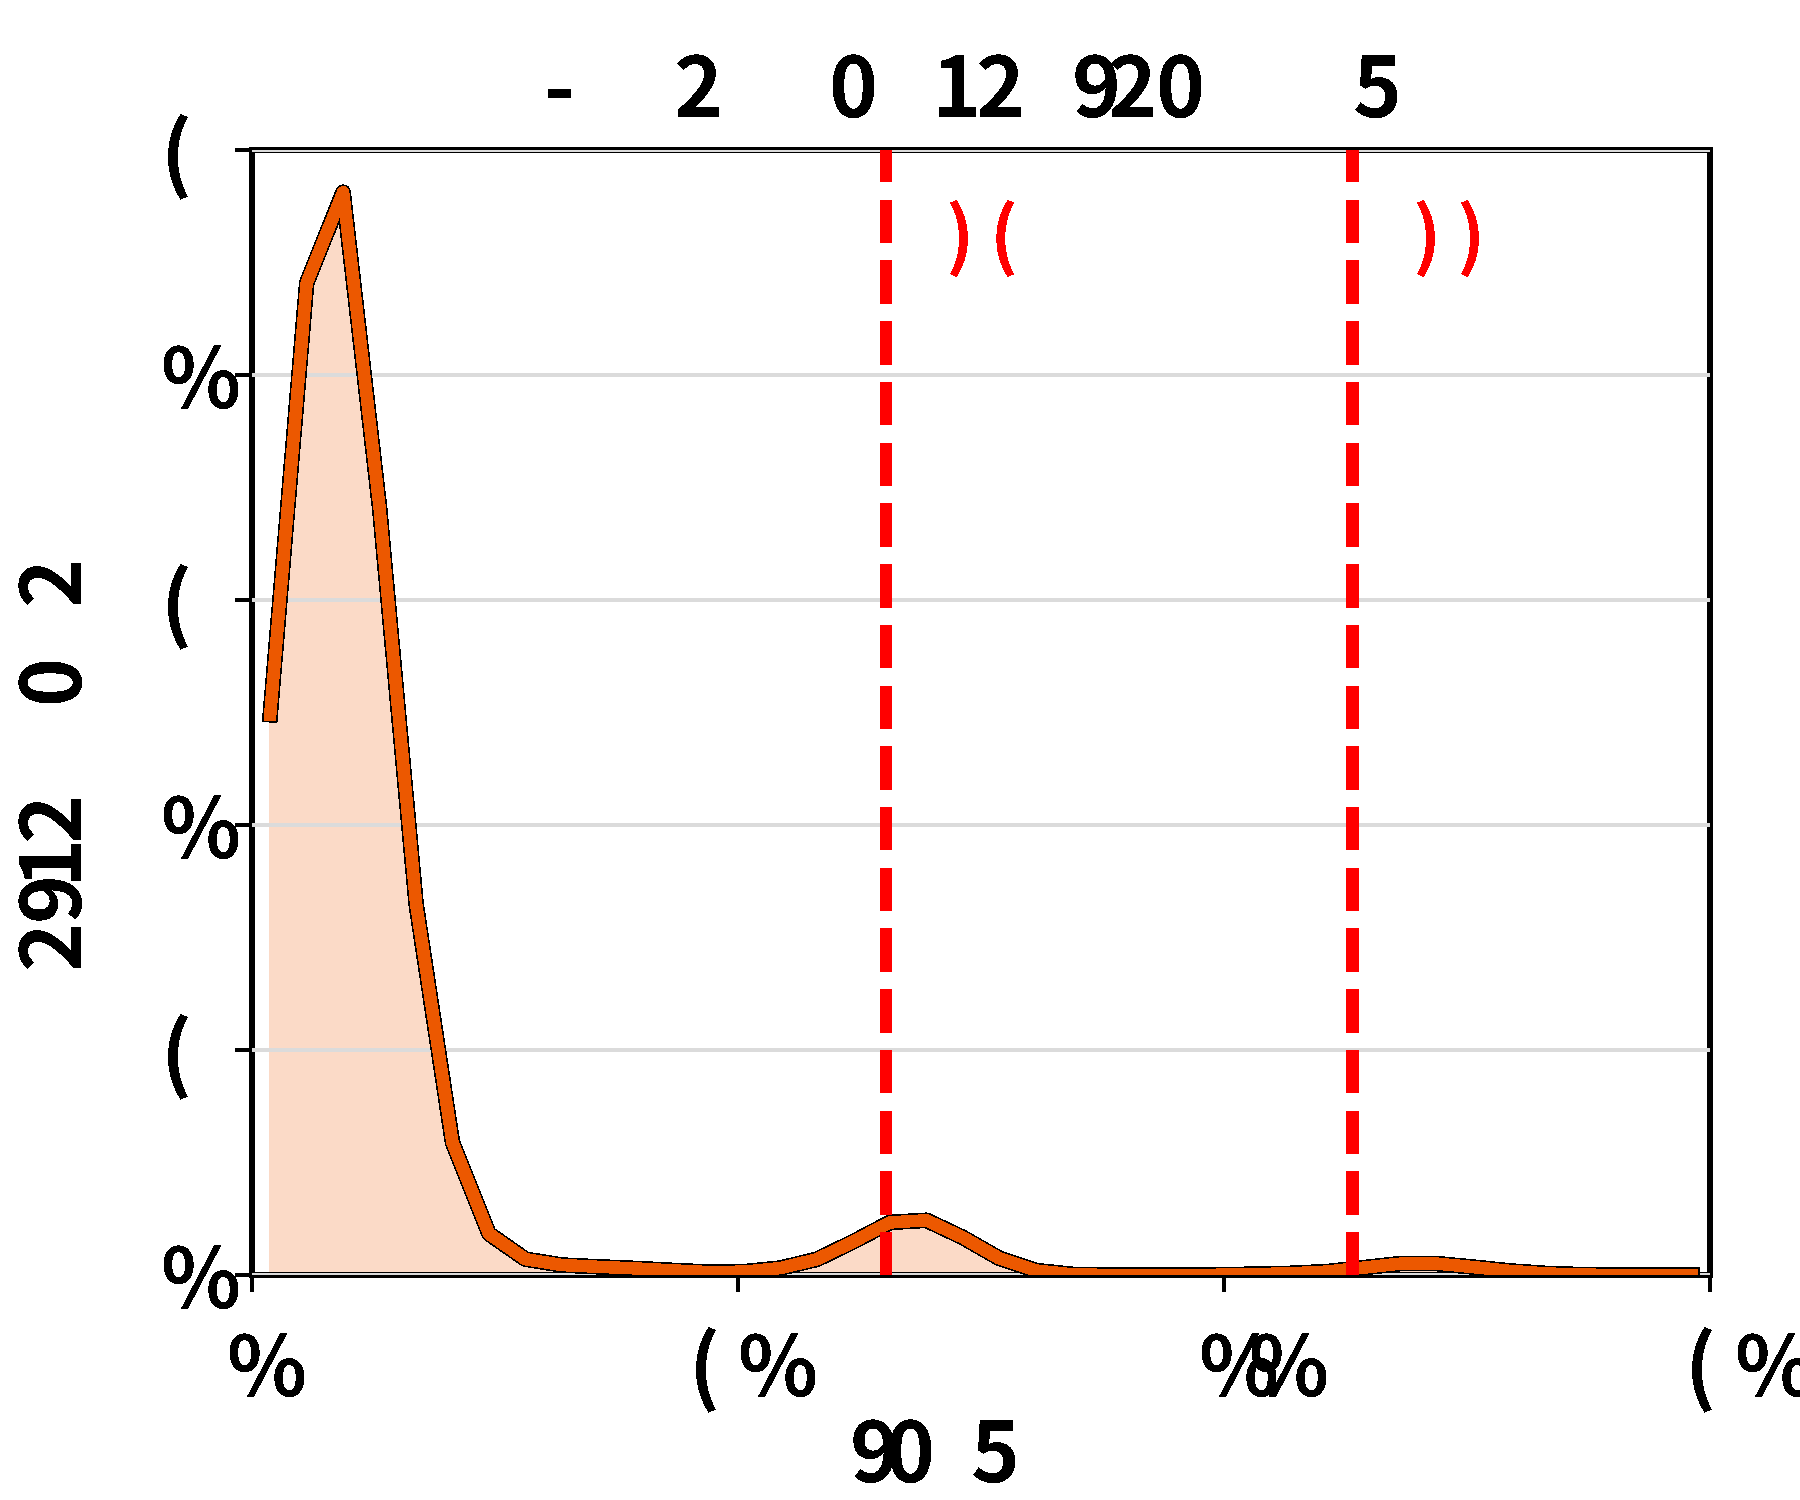
\includegraphics[width=0.8\linewidth ]{Figures/appendix_figs/hle_enhance_reasoning_latency_dist.pdf} % (b) optional
    \label{fig:hle_enhance_reasoning_latency}
  \end{subfigure}\hfill
  \begin{subfigure}[t]{0.32\textwidth}
    \centering
    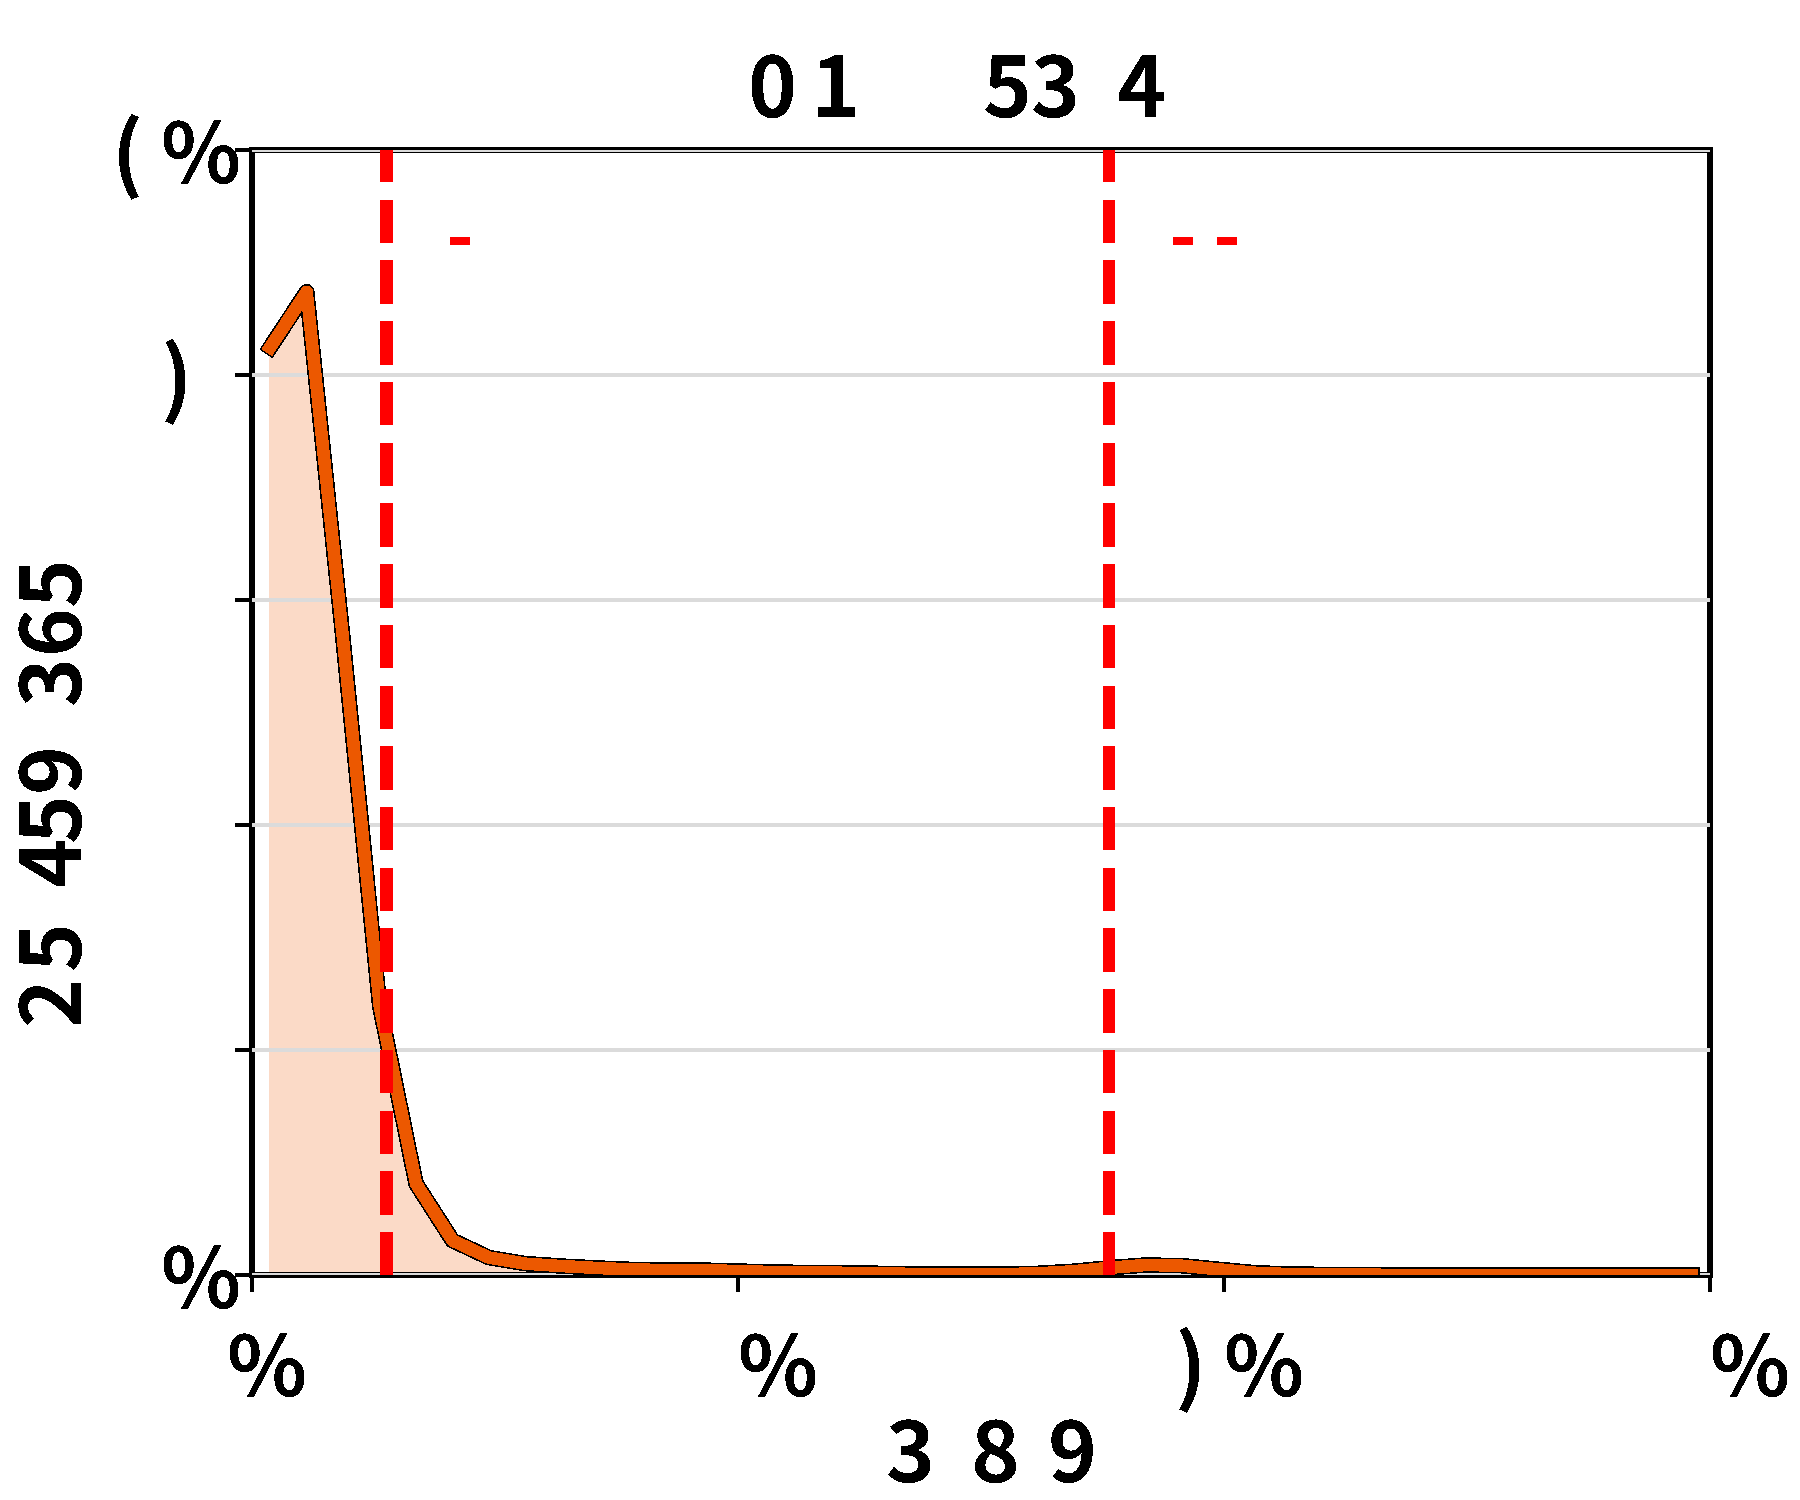
\includegraphics[width=0.8\linewidth ]{Figures/appendix_figs/hle_search_latency_dist.pdf} % (c) optional
    \label{fig:hle_search_latency}
  \end{subfigure}

  \vspace{2mm}

  % ===================== Row 2: SAB (now 3/3 filled) =====================
  \begin{subfigure}[t]{0.32\textwidth}
    \centering
    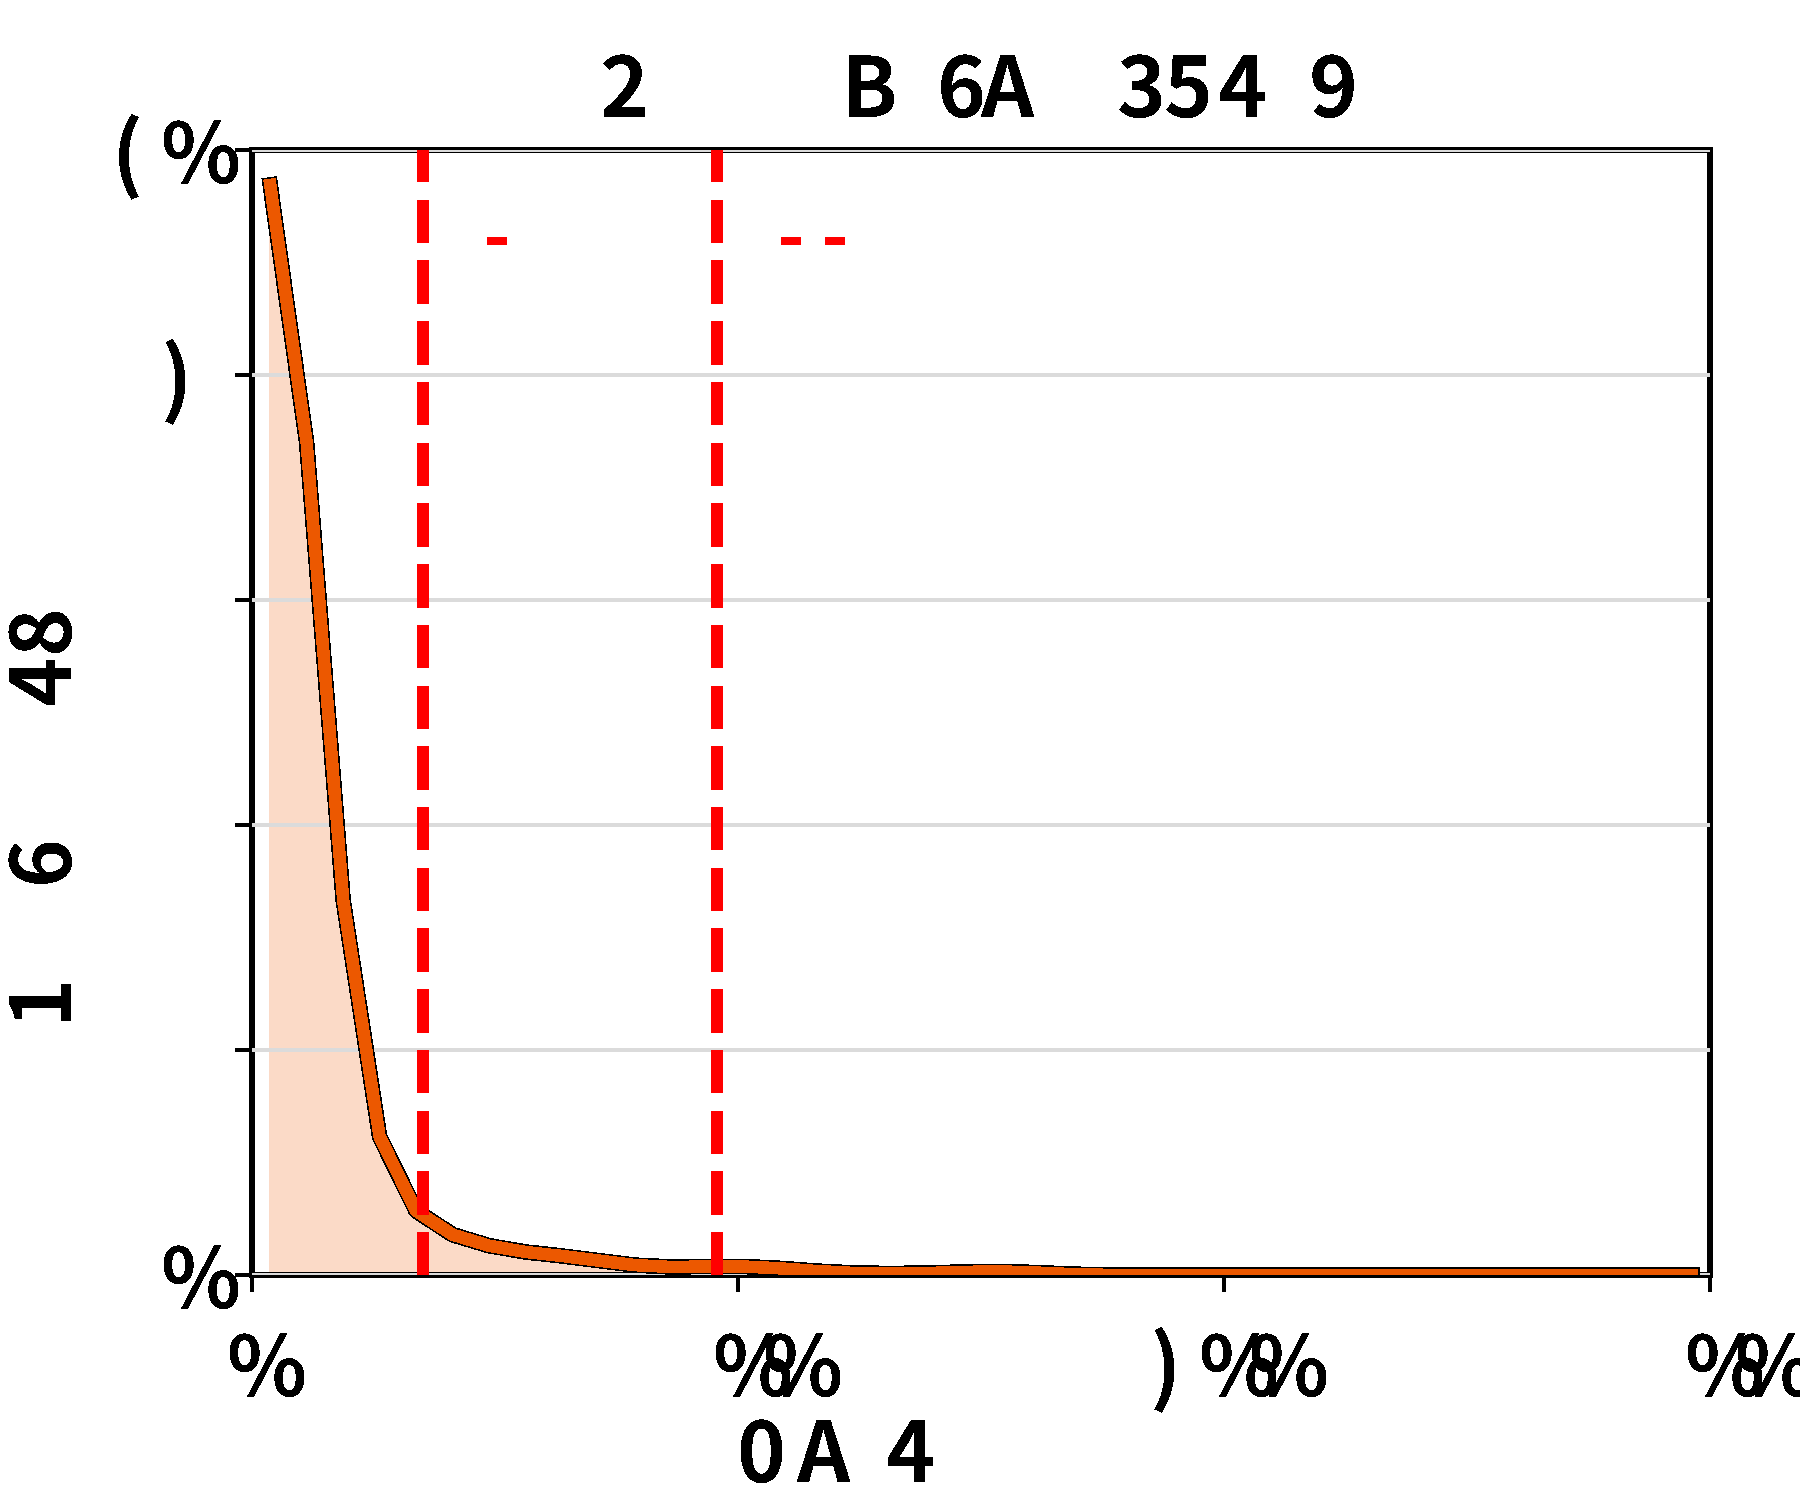
\includegraphics[width=0.8\linewidth ]{Figures/appendix_figs/sab_execute_bash_duration_dist.pdf} % (d) optional
    \label{fig:sab_execute_bash}
  \end{subfigure}\hfill
  \begin{subfigure}[t]{0.32\textwidth}
    \centering
    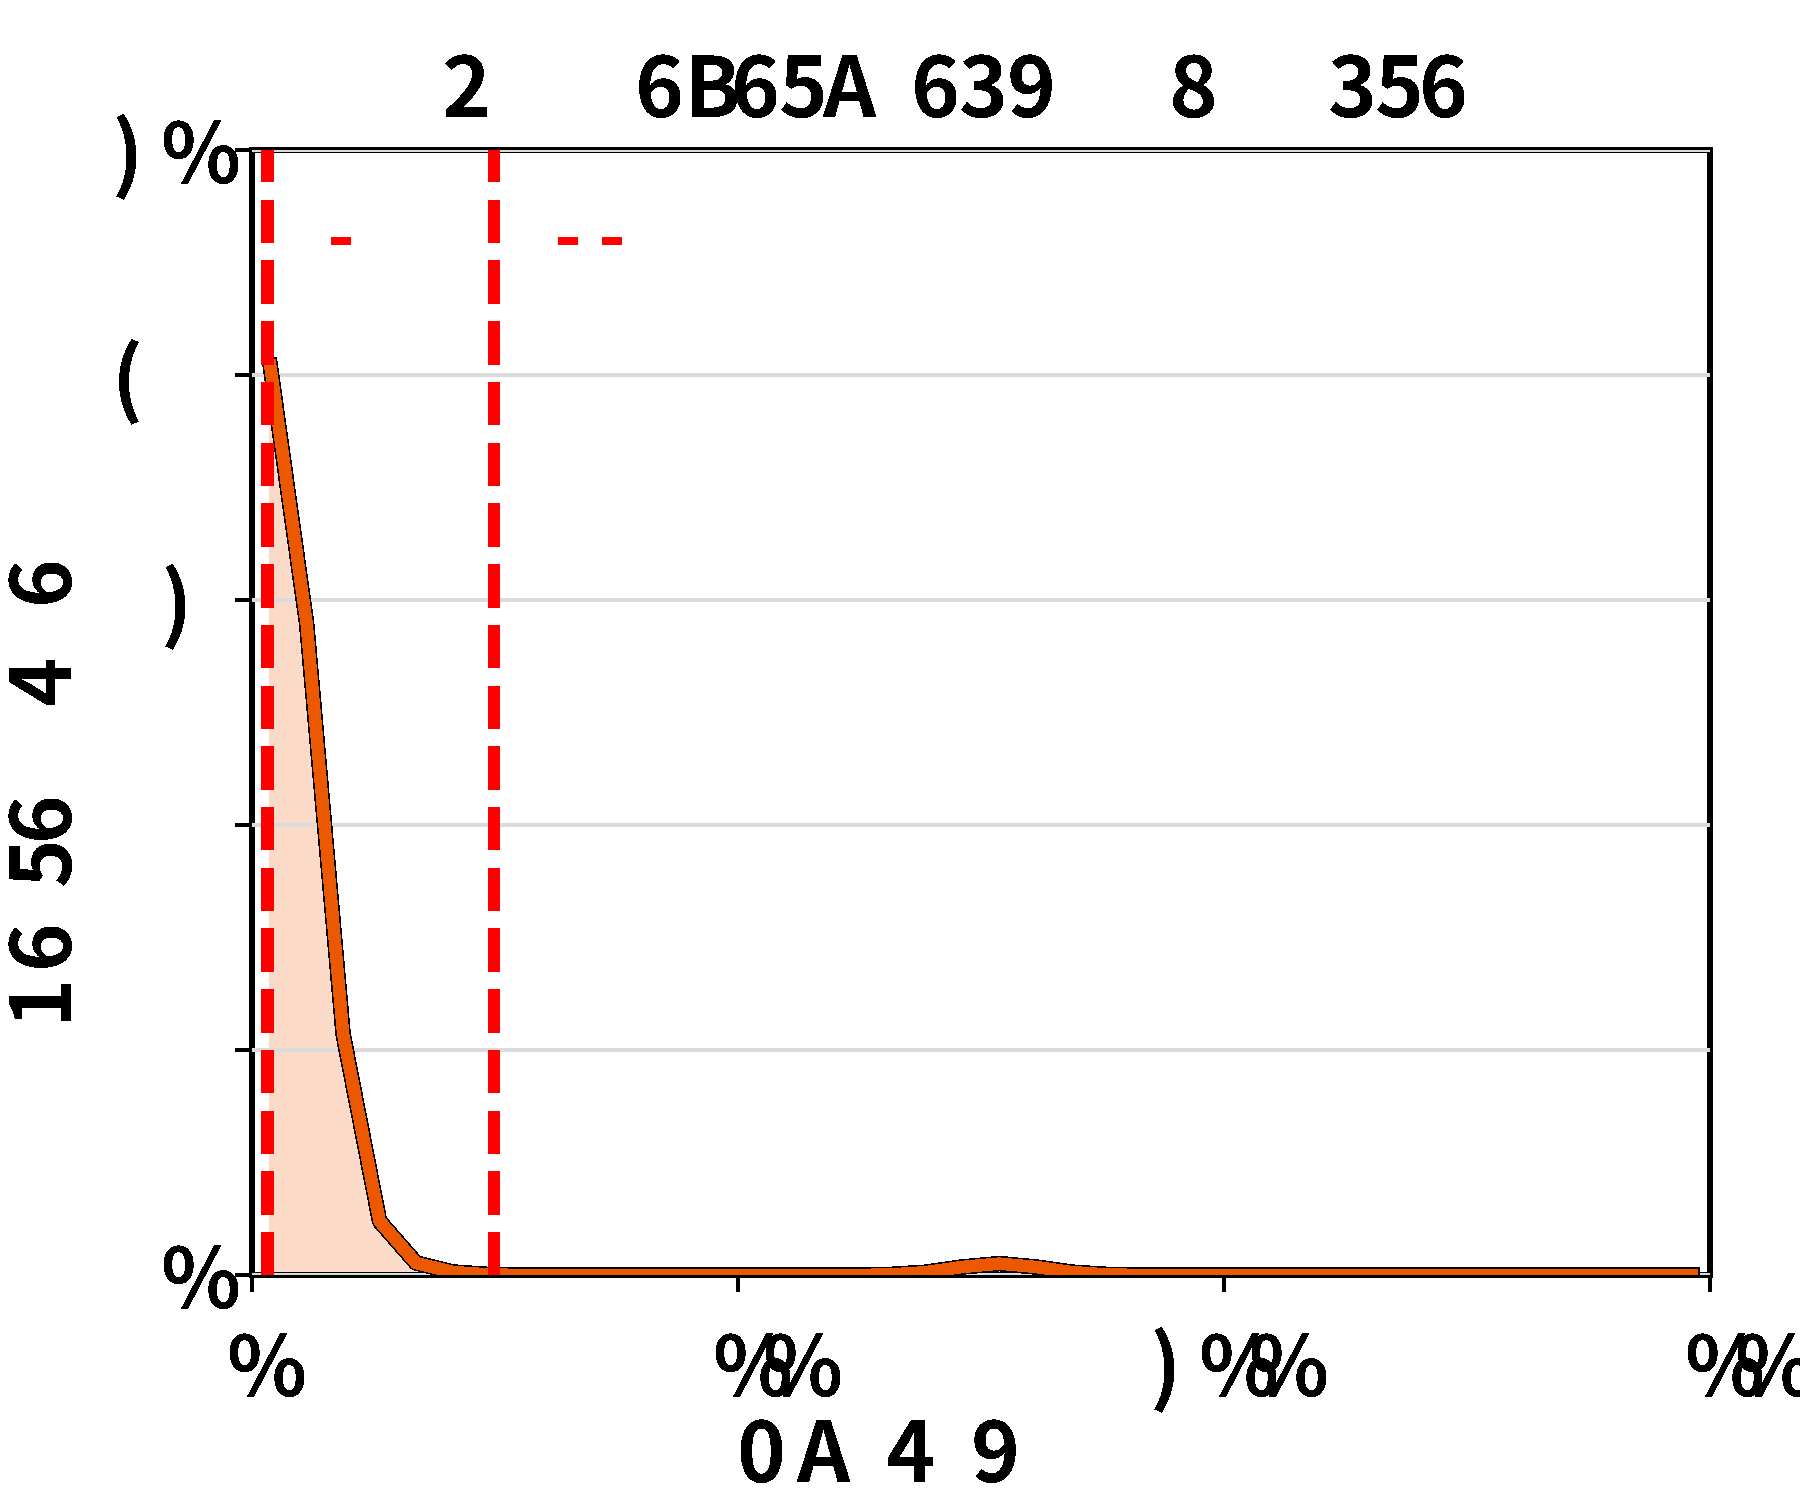
\includegraphics[width=0.8\linewidth ]{Figures/appendix_figs/sab_execute_ipython_cell_duration_dist.pdf} % (e) optional
    \label{fig:sab_execute_ipython}
  \end{subfigure}\hfill
  \begin{subfigure}[t]{0.32\textwidth}
    \centering
    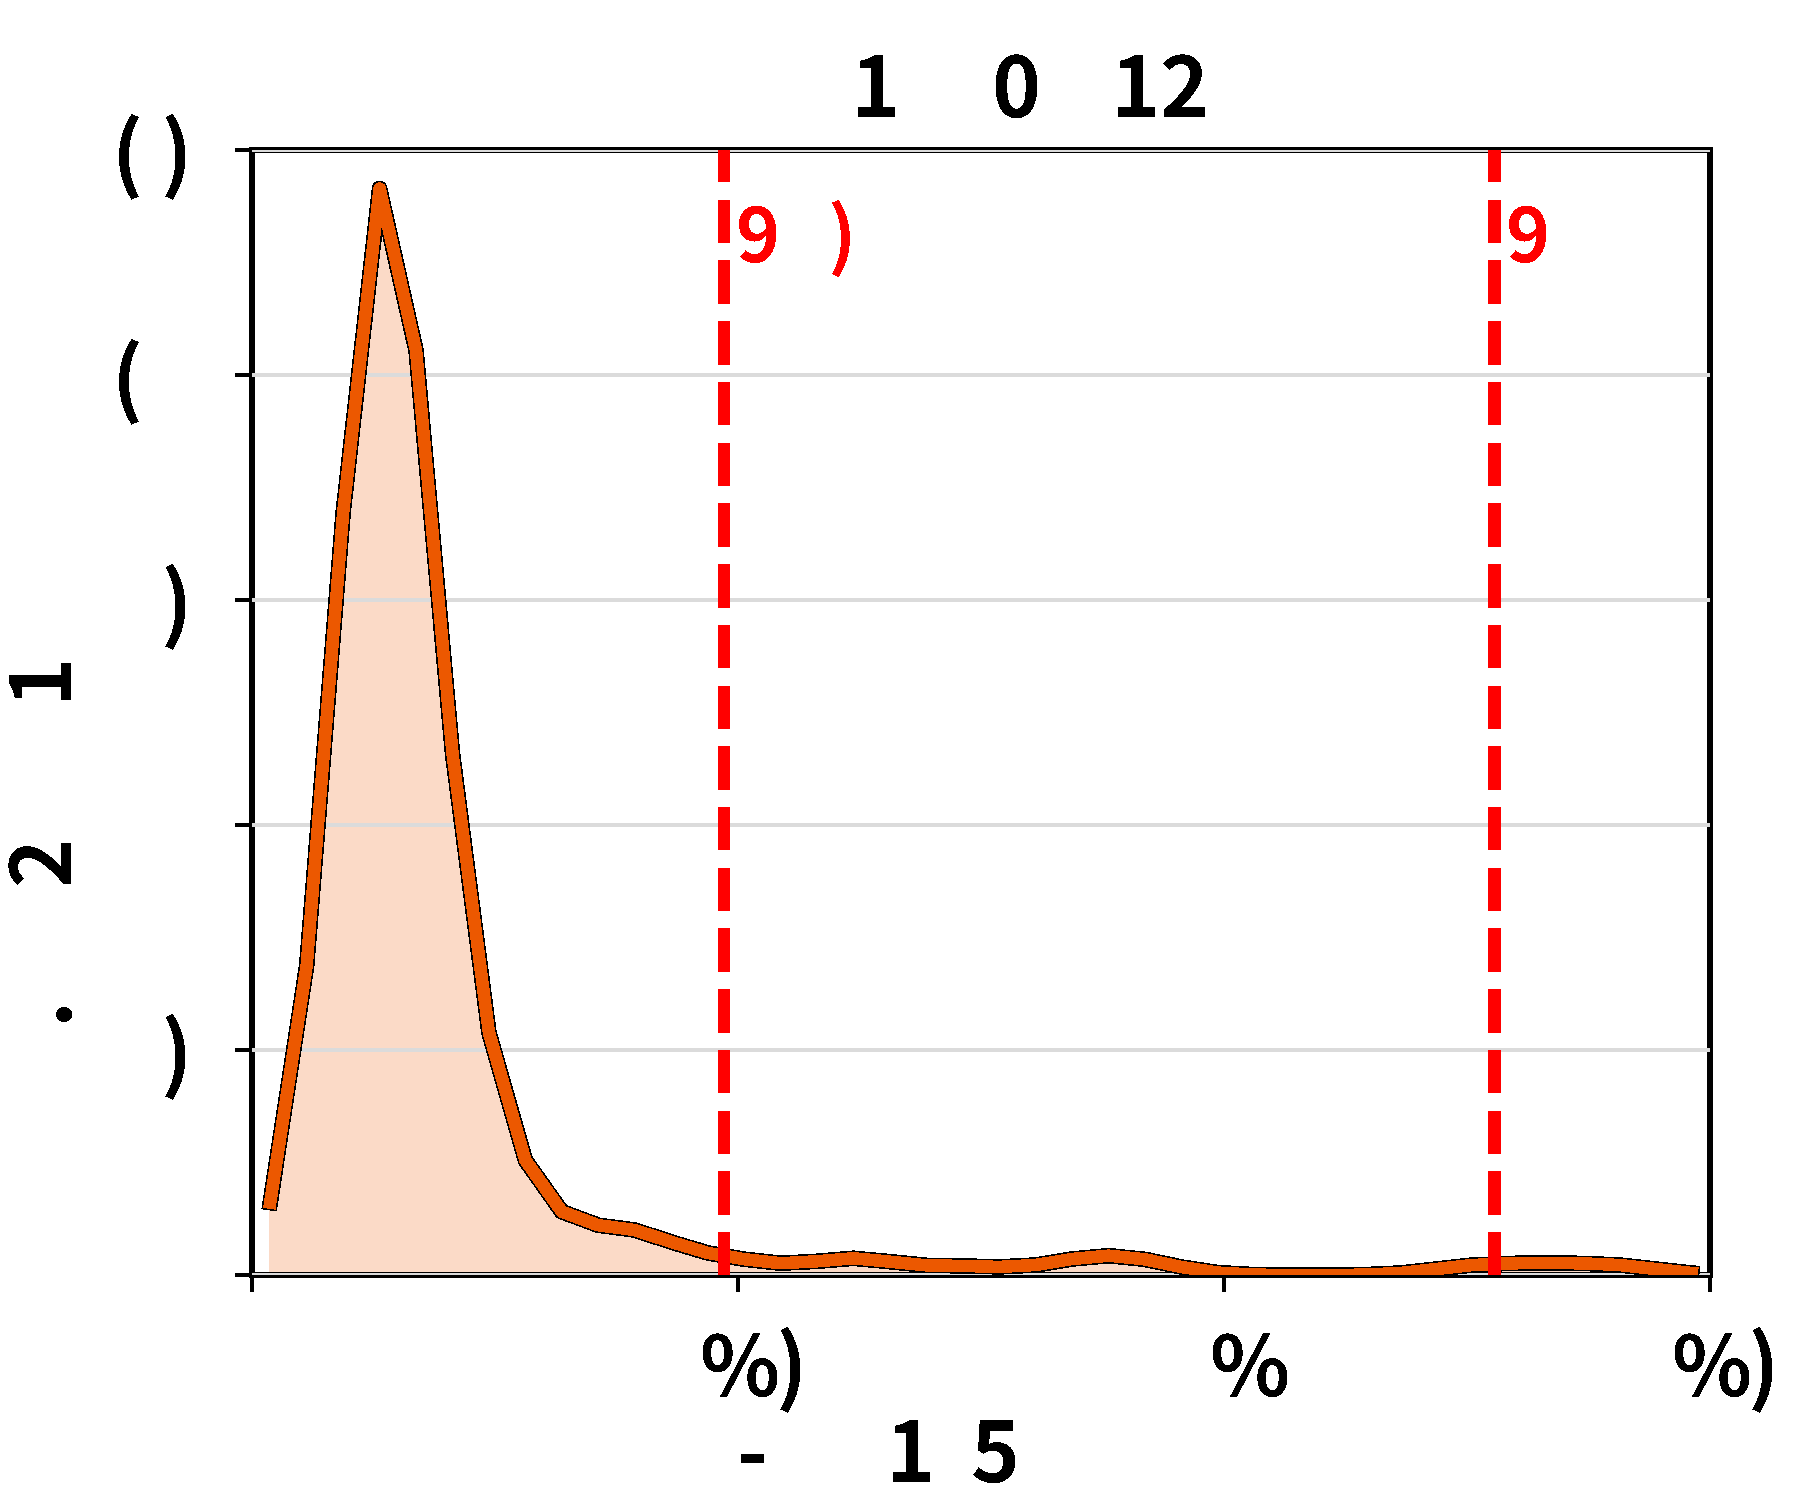
\includegraphics[width=0.8\linewidth ]{Figures/appendix_figs/sab_task_tracker_duration_dist.pdf}
    \label{fig:sab_task_tracker}
  \end{subfigure}

  \vspace{2mm}

  % ===================== Row 3: SAB (centered) =====================
  \begin{subfigure}[t]{0.32\textwidth}
    \centering
    % empty slot (keep layout)
    \label{fig:empty_slot_left}
  \end{subfigure}\hfill
  \begin{subfigure}[t]{0.32\textwidth}
    \centering
    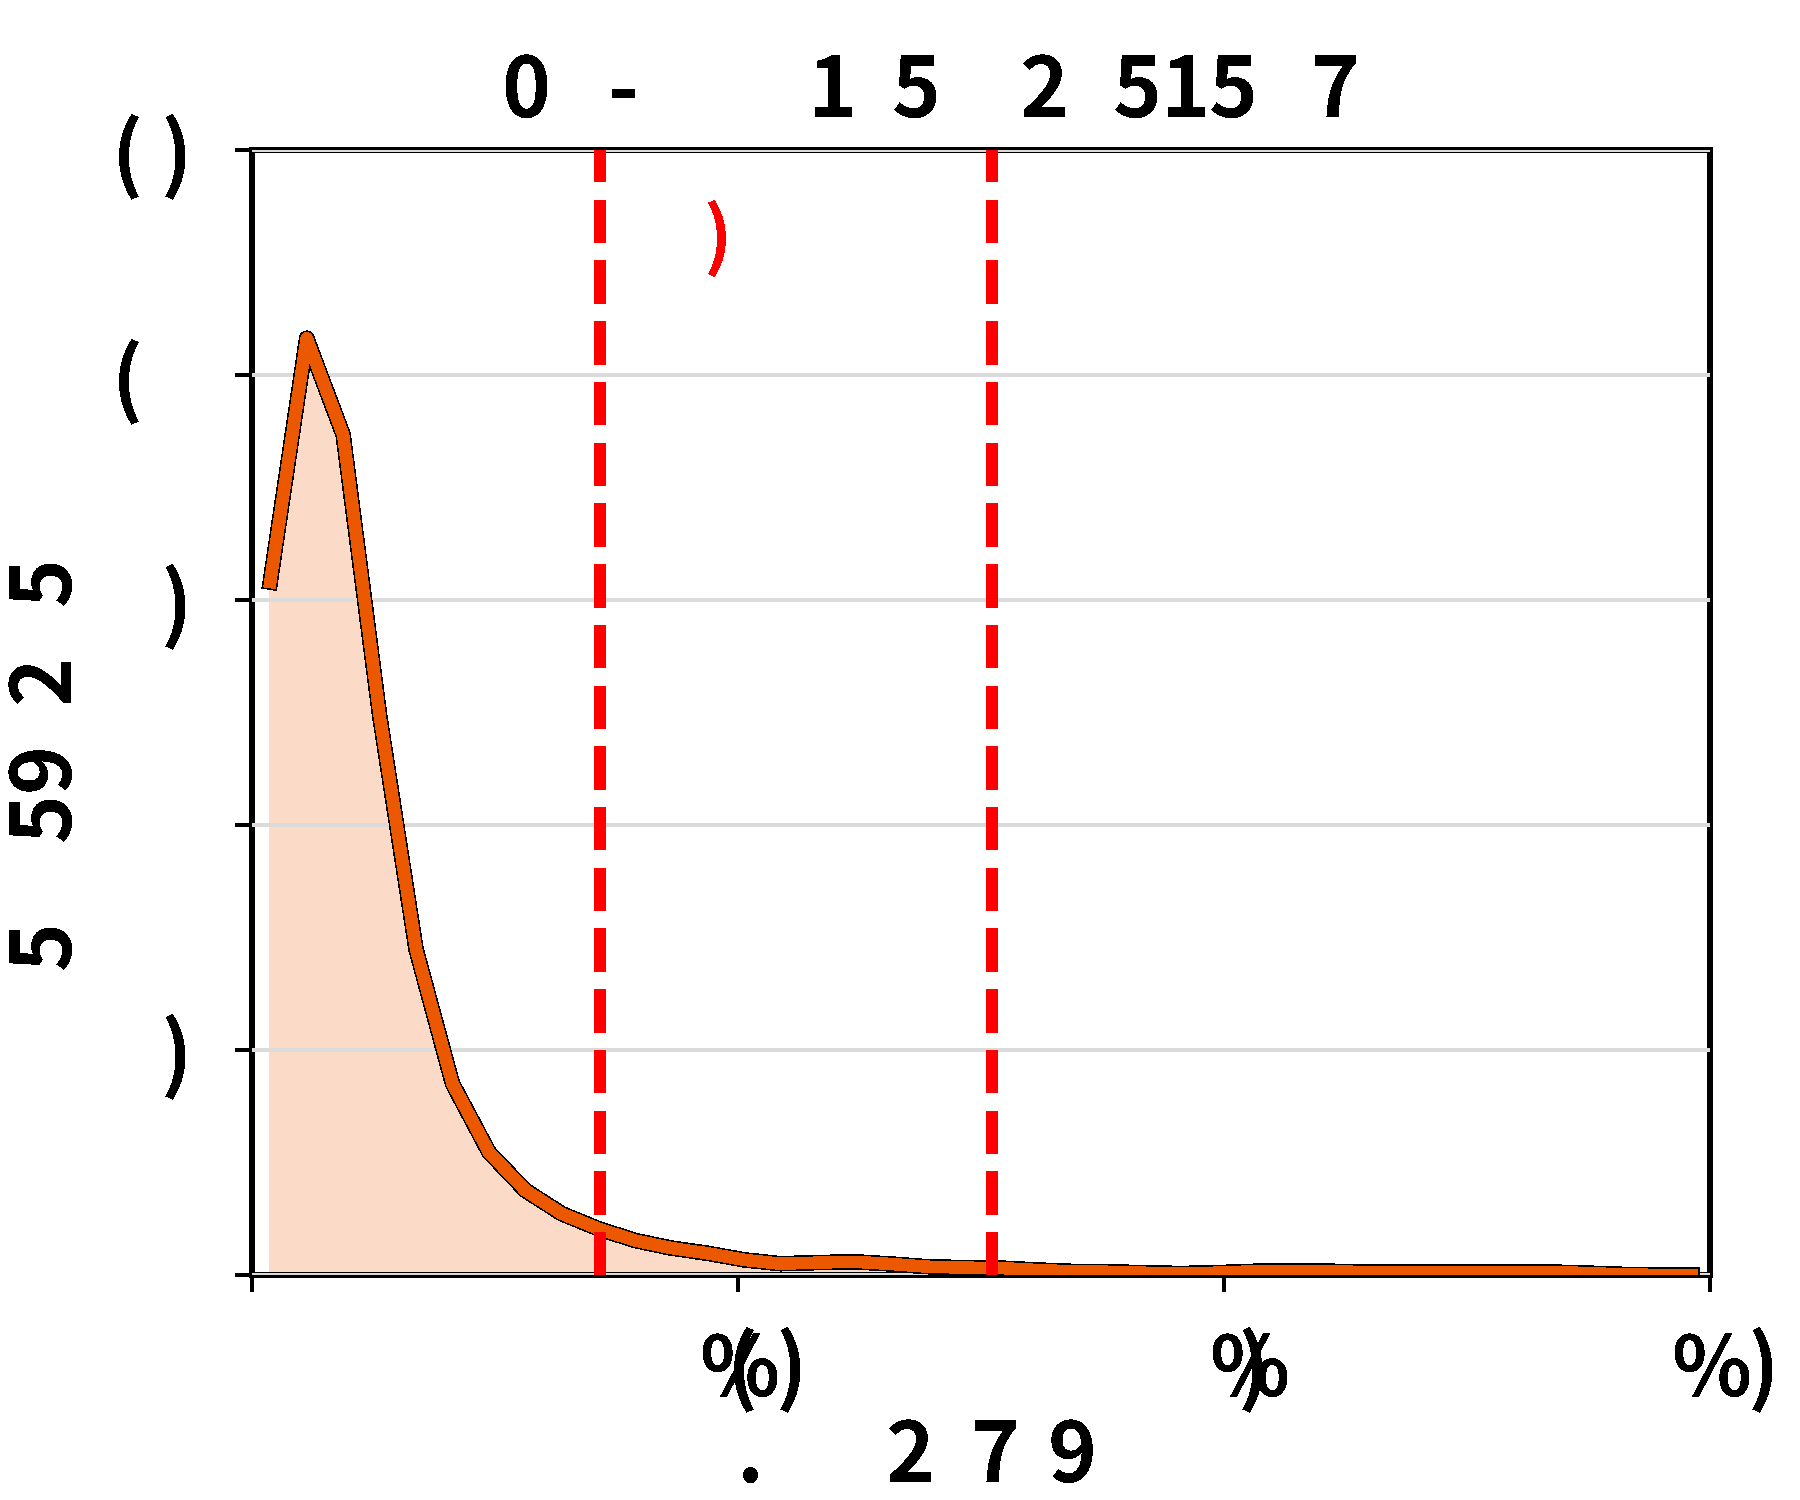
\includegraphics[width=0.8\linewidth]{Figures/appendix_figs/sab_str_replace_editor_duration_dist.pdf} % (f) optional
    \label{fig:sab_str_replace_editor}
  \end{subfigure}\hfill
  \begin{subfigure}[t]{0.32\textwidth}
    \centering
    % empty slot (keep layout)
    \label{fig:empty_slot_right}
  \end{subfigure}

  \caption{\textbf{Tool execution time distributions.}Tool execution time exhibits high variability and is difficult to predict.}

  \label{fig:tool_time}
\end{figure*}

\newpage
\section{KV cache hit rate statistics and interpretation}
\label{sec:kv_hit_rate_stats}

In our cost decomposition Equation~(\ref{eq:cost_decomp}), throughput loss in agentic serving mainly comes from \emph{non-productive} overheads:
KV re-computation induced by thrashing and idle KV caching during external tool execution, i.e.,
$\text{Cost}_{\text{recompute}}$ and $\text{Cost}_{\text{caching}}$. When tool calls are short and predictable, the acting phase occupies KV for only a short time, so $\text{Cost}_{\text{caching}}$ is small; thus, avoiding thrashing dominates: a higher KV cache hit rate typically implies fewer re-prefills and higher throughput.

However, when tool execution times are highly variable (see Appendix~\ref{app:tool_var}), a TTL-based scheduler can end up pinning the KV for long tool calls.
While this can reduce $\text{Cost}_{\text{recompute}}$ and thus increase the KV cache hit rate, it simultaneously inflates $\text{Cost}_{\text{caching}}$ and reduces throughput. This helps explain why continuum~\cite{li2025continuumefficientrobustmultiturn} can underperform on tool-heavy workloads despite achieving a higher KV cache hit rate (Figs.~\ref{fig:eval_infer_result},~\ref{fig:kv_hit_rate_data_statistics}).

\noindent\textbf{ThunderAgent adapts to these regimes by explicitly balancing caching and recomputation.}
ThunderAgent introduces a time-decay function $f(t)$ in Sec.~\ref{sec:scheduling_policy} for acting programs to trade off
$\text{Cost}_{\text{caching}}$ and $\text{Cost}_{\text{recompute}}$; we rigorously derive the optimal functional form of \(f(t)\) in Appendix~\ref{app:ft_discussion}.
By progressively lowering the effective memory priority of long-idle acting programs, the scheduler evicts their KV caches
to reduce idle caching cost while controlling recomputation, yielding better throughput in practice (Figs.~\ref{fig:eval_infer_result}).







\newpage
\section{Extended Theoretical Analysis.}

\subsection{Proof of Time Decay Function for Periodic Thrashing Detection.}
\label{app:ft_discussion}


\begin{hypothesis}[Unpredictable Tool Execution Time]
\label{hyp:unpredictable_tool}
For acting programs, we hypothesize that the scheduler cannot reliably predict the tool return time for a given program (see Appendix~\ref{app:tool_var}). Consequently, the decay function $f$ should depend only on the elapsed acting time $t$ in a time-homogeneous manner~\cite{parzen1999stochastic}.
\end{hypothesis}


\begin{hypothesis}[Boundary Conditions]
\label{hyp:boundary_conditions}
We assume the time decay function $f:[0,\infty)\rightarrow(0,1]$ satisfies
\begin{equation}
f(0) = 1, \lim_{t\to\infty} f(t) = 0,
\label{eq:boundary_f}
\end{equation}
An intuitive interpretation of these boundary conditions is that, when the tool execution time is $0$, corresponding to a multi-turn interaction without tool calls, all acting programs reduce to reasoning programs, and therefore $f(t)=1$. Conversely, if the tool execution time is infinite, the agentic workflow collapses to single-turn generation, akin to standard chatbot serving, since requests never return for the next-turn interactions. In this regime, setting $f(t)=0$ aligns the decay function with request-level scheduling policies.
\end{hypothesis}

\begin{theorem}[Admissible Time Decay Functions]
\label{thm:admissible_decay}
Under Hypothesis~\ref{hyp:unpredictable_tool} and \ref{hyp:boundary_conditions}, the admissible time decay function $f$ for our capacity check function in Equation~\ref{eq:time_decay} must take one of the following forms: exponential in continuous time, $f(t)=e^{-\lambda t}$ with $\lambda>0$, or geometric in discrete tick time, $f(k)=x^{-k}$ with $x>1$.
\end{theorem}

\begin{proof}
We prove this theorem by first formalizing the time-homogeneous property implied by
Hypothesis~\ref{hyp:unpredictable_tool}. Next, we inducing the admissible time decay functions $f$ under the boundary conditions in
Hypothesis~\ref{hyp:boundary_conditions}.
\smallskip

\noindent\textbf{Formalization of unpredictable tool time.} Let $t$ denote the elapsed acting time, measured in wall-clock time (continuous time) or in periodic-monitor ticks (discrete time). Under Hypothesis~\ref{hyp:unpredictable_tool}, the relative decay after waiting an additional duration $\Delta$ should not depend on the absolute elapsed time $t$, but only on the increment $\Delta$. We formalize this as the existence of a function $\phi:[0,\infty)\to(0,1]$ such that, for all $t,\Delta\ge 0$, \begin{equation} f(t+\Delta)=f(t)\,\phi(\Delta). \label{eq:time_homogeneous} \end{equation}

\noindent\textbf{Semigroup equation.} Setting $t=0$ in Equation~\ref{eq:time_homogeneous} and using the boundary condition $f(0)=1$
(from Hypothesis~\ref{hyp:boundary_conditions}) yields
$\phi(\Delta)=f(\Delta)$. Substituting back, we obtain the multiplicative
semigroup equation
\begin{equation}
f(t+\Delta)=f(t)\,f(\Delta),\qquad \forall t,\Delta\ge 0.
\label{eq:semigroup}
\end{equation}

\noindent \textbf{Continuous-time case (exponential decay).} We first consider the continuous-time case.
Define $h(t)\triangleq \ln f(t)$. Applying the logarithms on both sides of
Equation~\ref{eq:semigroup} yields the \emph{Cauchy functional equation}
\begin{equation}
h(t+\Delta)=h(t)+h(\Delta).
\label{eq:cauchy}
\end{equation}
Since $f(t)\in(0,1]$, we have $h(t)\le 0$ for all $t\ge 0$, which implies
that $h$ is bounded above on $[0,\infty)$. Under this boundedness condition, the Cauchy functional equation admits only linear solutions
of the form $h(t)=ct$ for some $c\in\mathbb{R}$. Writing $\lambda\triangleq -c\ge 0$,
we obtain
\begin{equation}
f(t)=e^{-\lambda t}.
\label{eq:exp_decay}
\end{equation}
Finally, the boundary condition $\lim_{t\to\infty} f(t)=0$
(Hypothesis~\ref{hyp:boundary_conditions}) rules out $\lambda=0$,
and thus $\lambda>0$.

\smallskip
\noindent \textbf{Discrete-time case (geometric decay).} We next consider the discrete-time setting, where elapsed acting time is
measured in integer ticks $k\in\mathbb{Z}_{\ge 0}$.
Equation~\ref{eq:semigroup} becomes
\begin{equation}
f(m+n)=f(m)\,f(n),\qquad \forall m,n\in\mathbb{Z}_{\ge 0}.
\label{eq:semigroup_discrete}
\end{equation}
Setting $n=1$ yields the recurrence $f(k)=f(k-1)f(1)$. Let $\gamma \triangleq f(1)$, we have
$f(k)=f(1)^k\triangleq \gamma^k$.
The boundary condition $\lim_{k\to\infty} f(k)=0$ implies $0<\gamma<1$.
Equivalently, we can parameterize
\begin{equation}
f(k)=x^{-k},\qquad x\triangleq \gamma^{-1}>1.
\label{eq:geom_decay}
\end{equation}

\noindent This completes the proof.
\end{proof}

\subsection{Proof of recomputation STP cost}
\label{app:prefill_stpcost}
As defined in \autoref{sec:utility_model}, the STP recomputation cost is given by:
\begin{equation}
    \text{Cost}_{\text{recompute}} = \int_{0}^{t_{recompute}} c_i(t) \, dt
\end{equation}
where $c_i(t)$ represents the instantaneous cost, which is proportional to the decoding step (i.e., $c_i(t) \propto t$). This proportionality arises because chunked prefill processes a constant number of KV pairs per iteration, resulting in a linear increase in accumulated computation over time. Consequently, evaluating the integral yields $\text{Cost}_{\text{recompute}} \propto t_{\text{recompute}}^2$. Given the relationship $t_{\text{recompute}} = c_i \times T_{\text{decode}} / \text{chunk}$, where both $T_{\text{decode}}$ and the chunk size are constant, it follows that:
\begin{equation*}
Cost_{\text{recompute}} \propto c_{i}^2
\end{equation*}

\subsection{Proof of minimized recomputation STP cost}

\label{app:_minimized_STP_cost}
We provide a rigorous proof for the optimality of the Shortest-First Eviction policy using an \textbf{exchange argument}.

\textbf{Problem Definition.}
We aim to select a subset of paused programs $S$ to evict such that the total reclaimed memory satisfies $\sum_{i \in S} c_i \ge \Delta C$, while minimizing the total re-computation cost $J(S) = \sum_{i \in S} c_i^2$. Note that the cost function $f(x) = x^2$ is strictly convex and super-additive (i.e., $(a+b)^2 > a^2 + b^2$ for positive $a, b$).

\textbf{Theorem.}
The optimal strategy to minimize $J(S)$ is to strictly select programs with the smallest context lengths $c_i$.

\textbf{Proof.}
Suppose, for the sake of contradiction, that the optimal set $S^*$ is \textit{not} the set of the shortest programs. This implies there exists a "long" program $p_{long} \in S^*$ and a "short" program $p_{short} \notin S^*$ (available but not selected) such that $c_{short} < c_{long}$.

We can construct a new set $S'$ by swapping or decomposing $p_{long}$. Since $c_{long} > c_{short}$, we can conceptualize $p_{long}$ as being composed of a segment of length $c_{short}$ and a residue $r = c_{long} - c_{short}$.

Replacing the selection of $p_{long}$ with $p_{short}$ (and theoretically the residue $r$) changes the cost. Consider the inequality derived from the convexity of the square function:
\begin{equation}
    c_{long}^2 = (c_{short} + r)^2 = c_{short}^2 + r^2 + 2 c_{short} r
\end{equation}
Since $c_{short} > 0$ and $r > 0$, the cross-term $2 c_{short} r > 0$. Therefore:
\begin{equation}
    c_{short}^2 + r^2 < c_{long}^2
\end{equation}

This inequality implies that breaking a large eviction target ($c_{long}$) into smaller components ($c_{short} + r$) strictly reduces the sum of squares.
In the context of our scheduler, this means that if we are satisfying the memory constraint $\Delta C$ using a large program, we can strictly decrease the penalty by swapping it for available smaller programs (or a combination thereof) that sum to the same capacity.

By iteratively applying this exchange—replacing the largest selected programs with smaller unselected programs—we monotonically decrease the cost function $J(S)$. The cost reaches its global minimum only when no such exchange is possible, i.e., when $S$ consists entirely of the programs with the smallest available context lengths.

\textbf{Conclusion.}
The Shortest-First strategy is globally optimal because the super-linear cost of attention ($O(L^2)$) penalizes fragmentation less than aggregation.

\newpage
\section{End-to-End Latency Analysis}
\label{app:e2e}
Though we have stated in \autoref{sec:intro} that program-level latency(time used for whole workflow generation) is far more important than end-to-end per step latency for autonomous agents and agentic RL rollout. Here we compare \ouralg's average per-step latency with vLLM and Continuum. \autoref{fig:e2e} shows that \ouralg significantly outperforms vLLM and Continuum when applying GLM4.6 and Qwen3 235B with mini-SWEAgent and Openhands on a single H100 serving in either low or high parallel workflow number. \textbf{The reason is that it seems to improve end-to-end latency by switching acting programs. But it actually delays all the running programs' latency by triggering heavy KV-cache thrashing.}




\begin{figure*}[]
  \centering
  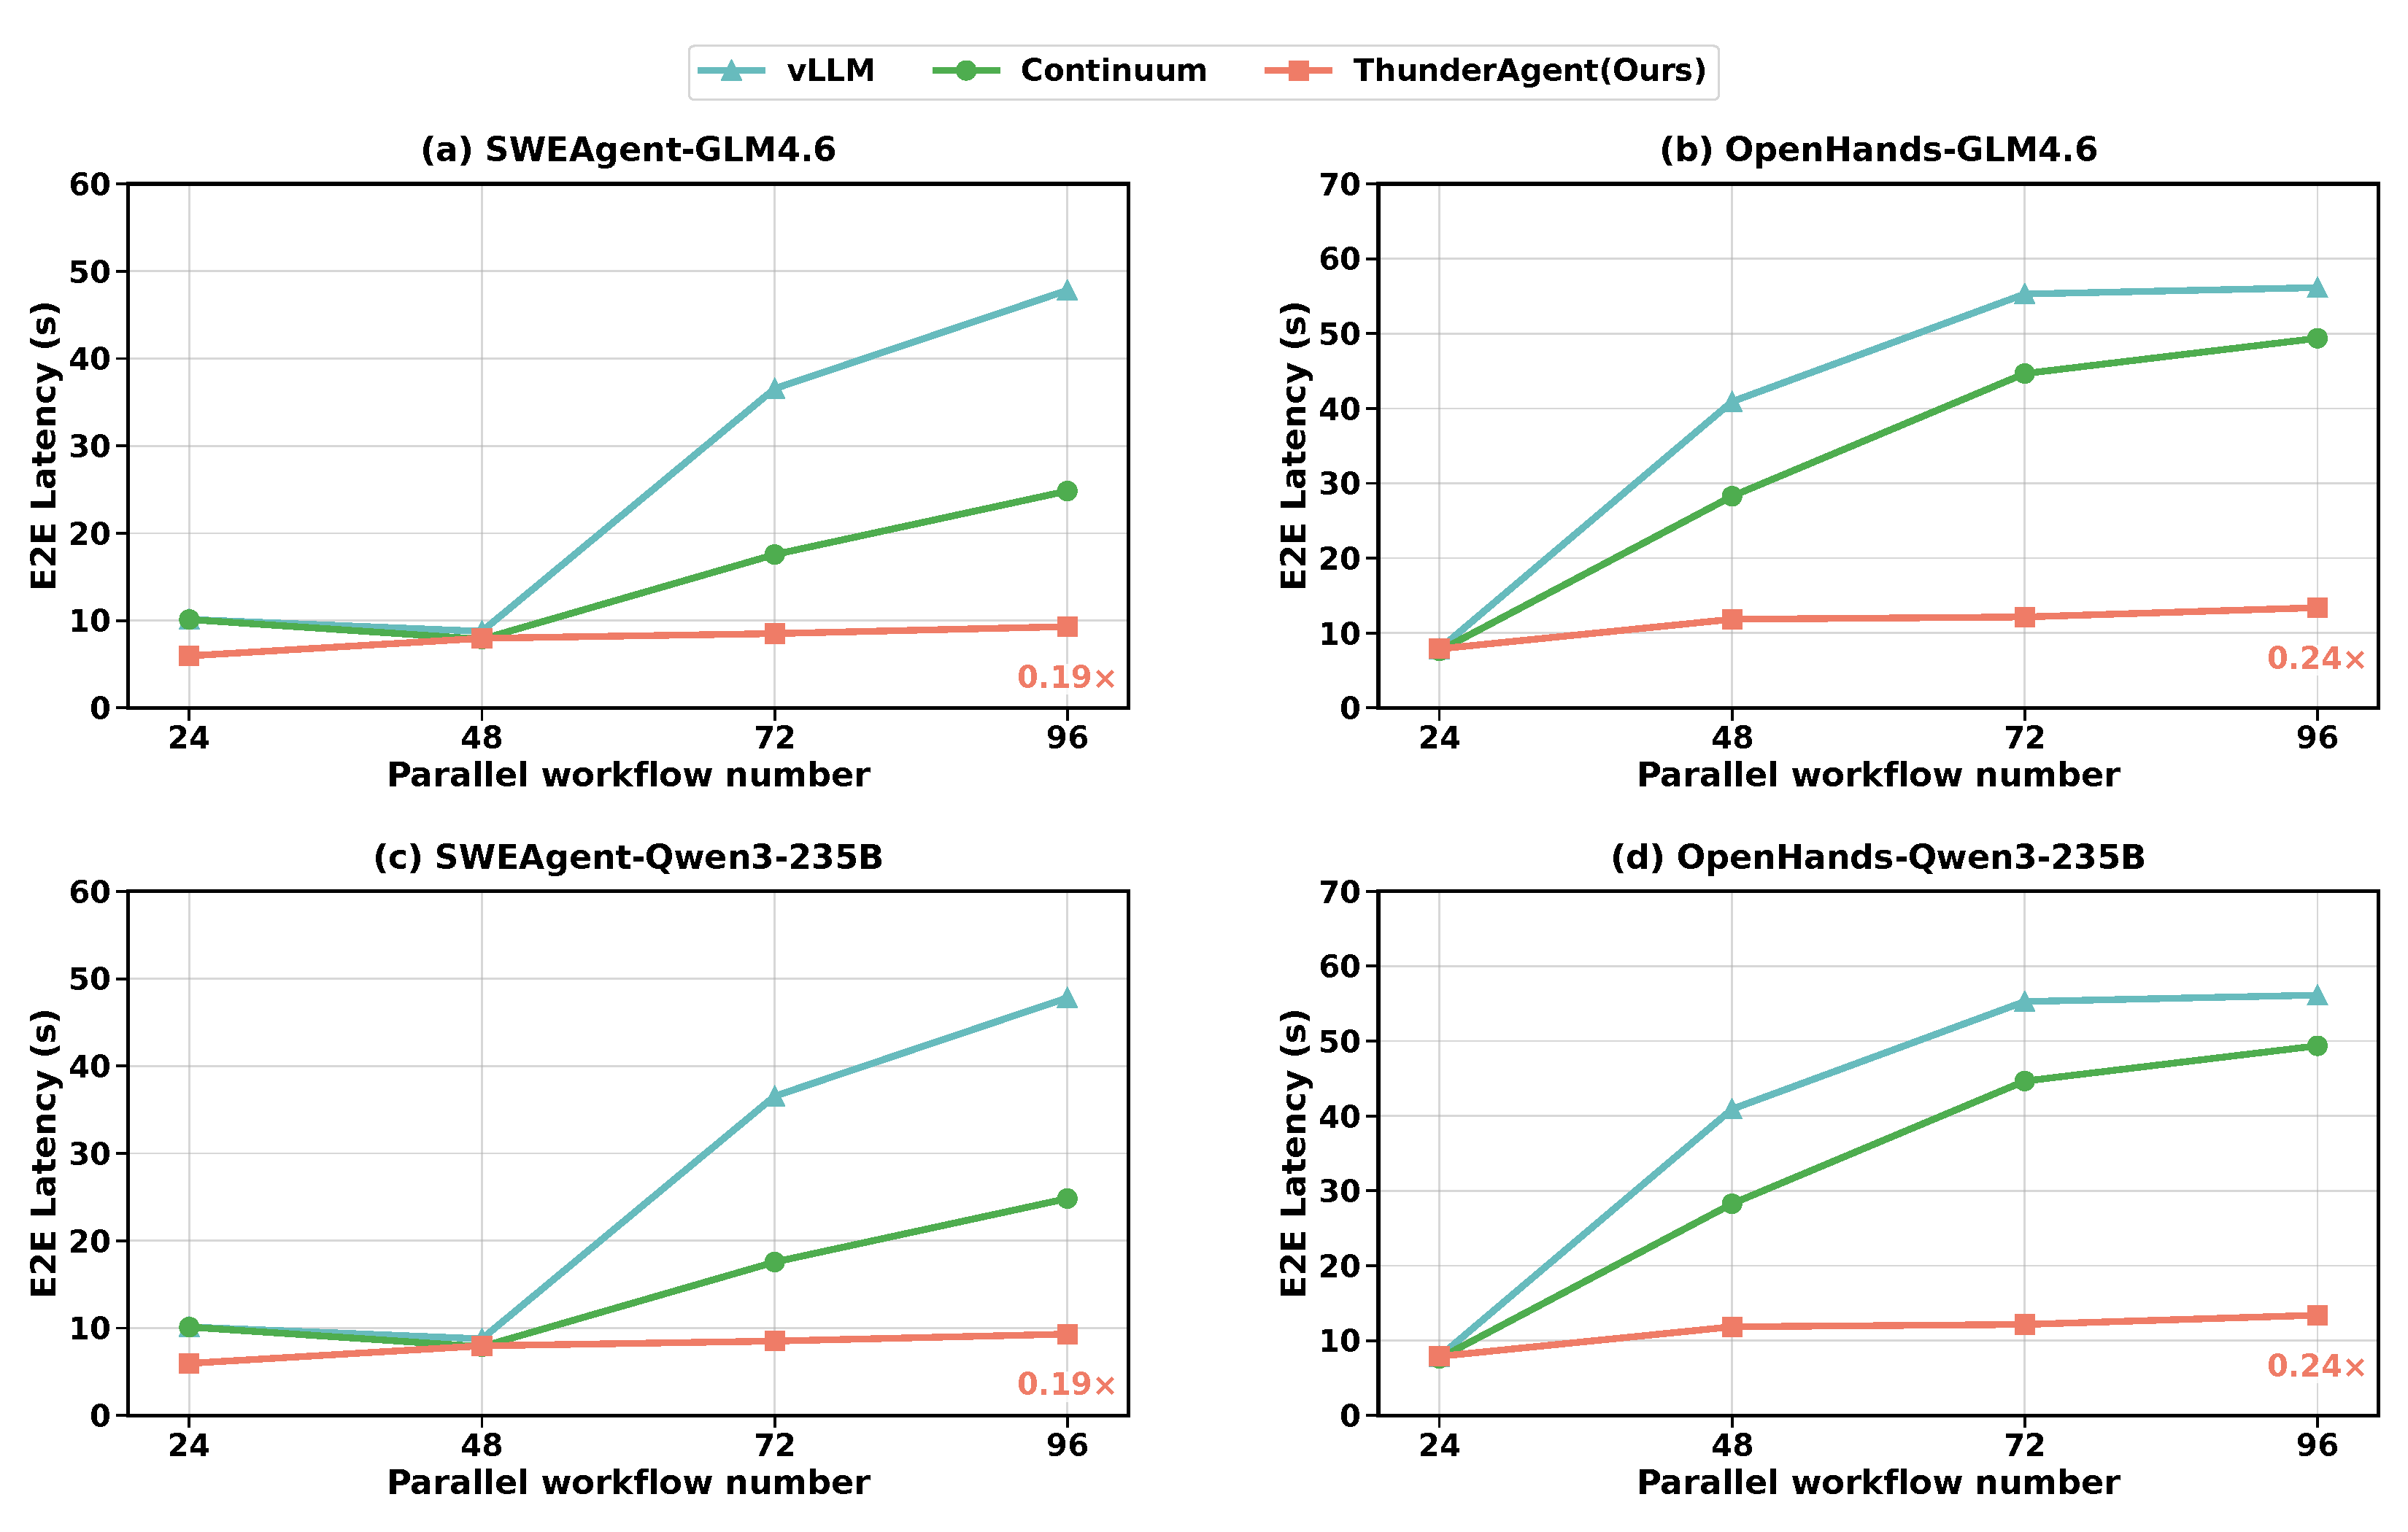
\includegraphics[width=0.7\textwidth]{Figures/latency_analysis_v4_final.pdf}
  \caption{End-to-End latency comparision}
  \label{fig:e2e}
\end{figure*}
% \begin{figure*}[!t]
%     \centering
%     \includegraphics[width=0.7·\columnwidth]{Figures/figure4_latency_reproduction.pdf}
%     \vspace{-2mm}
%     \caption{End-to-End latency comparision}
%     \label{fig:e2e}
% \vspace{-5mm}
% \end{figure*}

% You can have as much text here as you want. The main body must be at most $8$
% pages long. For the final version, one more page can be added. If you want, you
% can use an appendix like this one.

% The $\mathtt{\backslash onecolumn}$ command above can be kept in place if you
% prefer a one-column appendix, or can be removed if you prefer a two-column
% appendix.  Apart from this possible change, the style (font size, spacing,
% margins, page numbering, etc.) should be kept the same as the main body.
%%%%%%%%%%%%%%%%%%%%%%%%%%%%%%%%%%%%%%%%%%%%%%%%%%%%%%%%%%%%%%%%%%%%%%%%%%%%%%%
%%%%%%%%%%%%%%%%%%%%%%%%%%%%%%%%%%%%%%%%%%%%%%%%%%%%%%%%%%%%%%%%%%%%%%%%%%%%%%%
